%!TEX TS-program = xelatex
\documentclass[10pt,oneside]{article}
\usepackage[fontsize=9pt]{scrextend}

\usepackage[english]{babel}

\usepackage{amsmath,amssymb,amsfonts}
\usepackage[utf8]{inputenc}
\usepackage[T1]{fontenc}
\usepackage{stix2}
\usepackage[scaled]{helvet}
\usepackage[scaled]{inconsolata}

\usepackage{lastpage}

\usepackage{setspace}

\usepackage{ccicons}

\usepackage[hang,flushmargin]{footmisc}

\usepackage{geometry}

\setlength{\parindent}{0pt}
\setlength{\parskip}{6pt plus 2pt minus 1pt}

\usepackage{fancyhdr}
\renewcommand{\headrulewidth}{0pt}\providecommand{\tightlist}{%
  \setlength{\itemsep}{0pt}\setlength{\parskip}{0pt}}

\makeatletter
\newcounter{tableno}
\newenvironment{tablenos:no-prefix-table-caption}{
  \caption@ifcompatibility{}{
    \let\oldthetable\thetable
    \let\oldtheHtable\theHtable
    \renewcommand{\thetable}{tableno:\thetableno}
    \renewcommand{\theHtable}{tableno:\thetableno}
    \stepcounter{tableno}
    \captionsetup{labelformat=empty}
  }
}{
  \caption@ifcompatibility{}{
    \captionsetup{labelformat=default}
    \let\thetable\oldthetable
    \let\theHtable\oldtheHtable
    \addtocounter{table}{-1}
  }
}
\makeatother

\usepackage{array}
\newcommand{\PreserveBackslash}[1]{\let\temp=\\#1\let\\=\temp}
\let\PBS=\PreserveBackslash

\usepackage[breaklinks=true]{hyperref}
\hypersetup{colorlinks,%
citecolor=blue,%
filecolor=blue,%
linkcolor=blue,%
urlcolor=blue}
\usepackage{url}

\usepackage{caption}
\setcounter{secnumdepth}{0}
\usepackage{cleveref}

\usepackage{graphicx}
\makeatletter
\def\maxwidth{\ifdim\Gin@nat@width>\linewidth\linewidth
\else\Gin@nat@width\fi}
\makeatother
\let\Oldincludegraphics\includegraphics
\renewcommand{\includegraphics}[1]{\Oldincludegraphics[width=\maxwidth]{#1}}

\usepackage{longtable}
\usepackage{booktabs}

\usepackage{color}
\usepackage{fancyvrb}
\newcommand{\VerbBar}{|}
\newcommand{\VERB}{\Verb[commandchars=\\\{\}]}
\DefineVerbatimEnvironment{Highlighting}{Verbatim}{commandchars=\\\{\}}
% Add ',fontsize=\small' for more characters per line
\usepackage{framed}
\definecolor{shadecolor}{RGB}{248,248,248}
\newenvironment{Shaded}{\begin{snugshade}}{\end{snugshade}}
\newcommand{\KeywordTok}[1]{\textcolor[rgb]{0.13,0.29,0.53}{\textbf{#1}}}
\newcommand{\DataTypeTok}[1]{\textcolor[rgb]{0.13,0.29,0.53}{#1}}
\newcommand{\DecValTok}[1]{\textcolor[rgb]{0.00,0.00,0.81}{#1}}
\newcommand{\BaseNTok}[1]{\textcolor[rgb]{0.00,0.00,0.81}{#1}}
\newcommand{\FloatTok}[1]{\textcolor[rgb]{0.00,0.00,0.81}{#1}}
\newcommand{\ConstantTok}[1]{\textcolor[rgb]{0.00,0.00,0.00}{#1}}
\newcommand{\CharTok}[1]{\textcolor[rgb]{0.31,0.60,0.02}{#1}}
\newcommand{\SpecialCharTok}[1]{\textcolor[rgb]{0.00,0.00,0.00}{#1}}
\newcommand{\StringTok}[1]{\textcolor[rgb]{0.31,0.60,0.02}{#1}}
\newcommand{\VerbatimStringTok}[1]{\textcolor[rgb]{0.31,0.60,0.02}{#1}}
\newcommand{\SpecialStringTok}[1]{\textcolor[rgb]{0.31,0.60,0.02}{#1}}
\newcommand{\ImportTok}[1]{#1}
\newcommand{\CommentTok}[1]{\textcolor[rgb]{0.56,0.35,0.01}{\textit{#1}}}
\newcommand{\DocumentationTok}[1]{\textcolor[rgb]{0.56,0.35,0.01}{\textbf{\textit{#1}}}}
\newcommand{\AnnotationTok}[1]{\textcolor[rgb]{0.56,0.35,0.01}{\textbf{\textit{#1}}}}
\newcommand{\CommentVarTok}[1]{\textcolor[rgb]{0.56,0.35,0.01}{\textbf{\textit{#1}}}}
\newcommand{\OtherTok}[1]{\textcolor[rgb]{0.56,0.35,0.01}{#1}}
\newcommand{\FunctionTok}[1]{\textcolor[rgb]{0.00,0.00,0.00}{#1}}
\newcommand{\VariableTok}[1]{\textcolor[rgb]{0.00,0.00,0.00}{#1}}
\newcommand{\ControlFlowTok}[1]{\textcolor[rgb]{0.13,0.29,0.53}{\textbf{#1}}}
\newcommand{\OperatorTok}[1]{\textcolor[rgb]{0.81,0.36,0.00}{\textbf{#1}}}
\newcommand{\BuiltInTok}[1]{#1}
\newcommand{\ExtensionTok}[1]{#1}
\newcommand{\PreprocessorTok}[1]{\textcolor[rgb]{0.56,0.35,0.01}{\textit{#1}}}
\newcommand{\AttributeTok}[1]{\textcolor[rgb]{0.77,0.63,0.00}{#1}}
\newcommand{\RegionMarkerTok}[1]{#1}
\newcommand{\InformationTok}[1]{\textcolor[rgb]{0.56,0.35,0.01}{\textbf{\textit{#1}}}}
\newcommand{\WarningTok}[1]{\textcolor[rgb]{0.56,0.35,0.01}{\textbf{\textit{#1}}}}
\newcommand{\AlertTok}[1]{\textcolor[rgb]{0.94,0.16,0.16}{#1}}
\newcommand{\ErrorTok}[1]{\textcolor[rgb]{0.64,0.00,0.00}{\textbf{#1}}}
\newcommand{\NormalTok}[1]{#1}

\newlength{\cslhangindent}
\setlength{\cslhangindent}{1.5em}
\newlength{\csllabelwidth}
\setlength{\csllabelwidth}{3em}
\newenvironment{CSLReferences}[3] % #1 hanging-ident, #2 entry spacing
 {% don't indent paragraphs
  \setlength{\parindent}{0pt}
  % turn on hanging indent if param 1 is 1
  \ifodd #1 \everypar{\setlength{\hangindent}{\cslhangindent}}\ignorespaces\fi
  % set entry spacing
  \ifnum #2 > 0
  \setlength{\parskip}{#2\baselineskip}
  \fi
 }%
 {}
\usepackage{calc} % for \widthof, \maxof
\newcommand{\CSLBlock}[1]{#1\hfill\break}
\newcommand{\CSLLeftMargin}[1]{\parbox[t]{\maxof{\widthof{#1}}{\csllabelwidth}}{#1}}
\newcommand{\CSLRightInline}[1]{\parbox[t]{\linewidth}{#1}}
\newcommand{\CSLIndent}[1]{\hspace{\cslhangindent}#1}\usepackage[table,dvipsnames]{xcolor}

\geometry{includemp,
            letterpaper,
            top=2.4cm,
            bottom=2.4cm,
            left=1.0cm,
            right=1.0cm,
            marginparwidth=5cm,
            marginparsep=1.0cm}

\usepackage[singlelinecheck=off]{caption}

\captionsetup{
  font={small},
  labelfont={bf},
  format=plain,
  labelsep=quad
}

\usepackage{floatrow}

\floatsetup[figure]{margins=hangright,
              facing=no,
              capposition=beside,
              capbesideposition={center,outside},
              floatwidth=\textwidth}

% \floatsetup[table]{margins=hangright,
%              facing=no,
%              capposition=beside,
%              capbesideposition={center,outside},
%              floatwidth=\textwidth}

\pagestyle{plain}

\setcounter{secnumdepth}{5}

\usepackage{titlesec}

\titleformat{\section}[block]
{\normalfont\large\sffamily}
{\thesection}{.5em}{\titlerule\\[.8ex]\bfseries}

\titleformat{\subsection}[runin]
{\normalfont\fontseries{b}\selectfont\filright\sffamily}
{\thesubsection.}{.5em}{}

\titleformat{\subsubsection}[runin]
{\normalfont\itshape\rmfamily\bfseries}{\thesubsubsection}{1em}{}

\fancypagestyle{firstpage}
{
   \fancyhf{}
   \renewcommand{\headrulewidth}{0pt}
   \fancyfoot[R]{\footnotesize\ccby}
   \fancyfoot[L]{\footnotesize\sffamily\today}
}

\fancypagestyle{normal}
{
  \fancyhf{}
  \fancyfoot[R]{\footnotesize\sffamily\thepage\ of \pageref*{LastPage}}
}

\usepackage{tikz}
\begin{document}
\pagestyle{normal}
\thispagestyle{firstpage}

\newcommand{\colorRule}[3][black]{\textcolor[HTML]{#1}{\rule{#2}{#3}}}

\noindent {\LARGE \textbf{\textsf{Thesis proposal}}}

\medskip
\begin{flushleft}
{\small
%
\href{https://orcid.org/0000-0002-6506-6487}{Michael D.\,Catchen}%
%
\,\textsuperscript{1,2}
\vskip 1em
\end{flushleft}

\vskip 2em
\makebox[0pt][l]{\colorRule[CCCCCC]{2.0\textwidth}{0.5pt}}
\vskip 2em
\noindent



The proposal for my thesis, \emph{Simulation models for predictive
ecology}




\vskip 2em
\makebox[0pt][l]{\colorRule[CCCCCC]{2.0\textwidth}{0.5pt}}
\vskip 2em

\hypertarget{introduction}{%
\section{Introduction}\label{introduction}}

Within the last several hundred years, human activity has induced rapid
changes in Earth's atmosphere, oceans, and surface. Greenhouse gas
emissions have caused an increase the temperature of both Earth's
terrain and oceans, and both agricultural and urban development has
rapidly reshaped the Earth's land cover. These the bulk of this change
has occurred within the last several hundred years, a geological
instant, inducing a sudden shift in conditions to Earth's climate and
biosphere. As a result \emph{ecological forecasting}---modeling how
ecosystems and their services will change in the future---and then using
these forecasts to make decisions to mitigate the negative consequences
of this change on ecosystems, their functioning, and the services they
provide to humans has emerged as an imperative for ecology and
environmental science (Dietze 2017). However, robust prediction of
ecological processes is, to say the least, quite difficult (Beckage
\emph{et al.} 2011; Petchey \emph{et al.} 2015). This difficultly is
compounded by a few factors, the first being that sampling ecosystems is
not easy. Ecological data is often biased, noisey, and sparse in both
space and time. The current paucity of ecological data has resulted in
much interest in developing global systems for \emph{ecosystem
monitoring} (Makiola \emph{et al.} 2020), which would systematize the
collection of biodiversity data in manner that makes detecting and
predicting change more possible than at the moment (Urban \emph{et al.}
2021).

The second major challenge in ecological forecasting is that the
underlying dynamics of most ecological processes are unknown and instead
must be inferred from this (sparse) data. Much of the history of
quantitatively modeling ecosystems have been done in the language of
dynamical systems, describing how the value of an observable state of
the system, represented by a vector of numbers
\([x_1, x_2, \dots, x_n]^T = \vec{x}\) changes as over time, yielding
models in the form of differential equations in continuous-time
settings, \(\frac{dx}{dt} = f(x)\), or difference equations in
discrete-time settings, \(x_t = f(x_{t-1})\), where
\(f:\mathbb{R}^n \to \mathbb{R}^n\) is an arbitrary function describing
how the system changes on a moment-to-moment basis (e.g.~in the context
of communities, \(f\) could be Lotka-Voltera, Holling-Type-III or
DeAngelis-Beddington functional response). The form of this functional
response in real systems, and whether it is meaningfully non-zero for a
given species interaction, is effectively unknown, and some forms are
inherently more ``forecastable'' than others (Beckage \emph{et al.}
2011; Chen \emph{et al.} 2019; Pennekamp \emph{et al.} 2019). The
initial success of these forms of models can be traced back to the
larger program of ontological reductionism, which became the default
approach to modeling in the sciences after its early success in physics,
which, by the time ecology was becoming a quantitative science (sometime
in the 20th century, depending on who you ask), became the foundation
for mathematical models in ecology.

However, we run into many problems when aiming to apply this type of
model to empirical ecological data. Ecosystems are perhaps the
quintessential example of system that cannot be understood by iterative
reduction of its components into constituent parts---ecological
phenomena are emergent: the product of different mechanisms operating a
different spatial, temporal, and organizational scales (Levin 1992).
Further this analytical approach to modeling explicitly ignores known
realities: ecological dynamics not deterministic and many analytic
models in ecology assume long-run equilibrium. Finally, perhaps the
biggest challenge in using these models to describe ecological processes
is ecosystems consist of more dimensions than the tools of analytic
models are suited for. As the number of variables in an analytic model
increases, so does the ability of the scientist to discern clear
relationships between them given a fixed amount of data, the so-called
``curse'' of dimensionality.

But these problems are not solely unique to ecology. The term
\emph{ecological forecasting} implicitly creates an analogy with weather
forecasting. Although it has become a trite joke to complain about the
weather forecast being wrong, over the least 50 years the field of
numerical weather prediction (NWP) has dramatically improved out ability
to predict weather across the board (Bauer \emph{et al.} 2015). The
success of NWP, and the Earth observations systems that support it (Hill
\emph{et al.} 2004), should serve as a template for development of a
system for monitoring Earth's biodiversity. Much like ecology, NWP is
faced with high-dimensional systems that are governed by different
mechanisms at different scales. The success of NWP is that, rather than,
say, attempt to forecast the weather in Quebec by applying Navier-Stokes
to entire province, to instead use simulation models which describe
known mechanisms at different scales, and use the availability to
increasing computational power to directly simulate many batches of
dynamics which directly incorporate stochasticity and uncertainty in
parameter estimates via random number generation.

But forecasting is only half the story---if indeed ``{[}ecologists{]}
have hitherto only interpreted the world in various ways; the point is
to change it,'' then once we have a forecast about how an ecosystem will
change in the future, what if this forecast predicts a critical
ecosystem service will deteriorate? We are still left with the question,
what do we in the time being to mitigate the potentially negative
consequences a forecast predicts? In this framing, mitigating the
consequences of anthropogenic change on ecosystems becomes an
optimization problem: given a forecast of the future state of the
system, and some ``goal'' state for the future, the problem is then to
optimize our intervention into the system to maximize the probability
the system approaches our ``goal'' state. This dissertation aims to this
framework for ecosystem monitoring and forecasting
(fig.~\ref{fig:thesis}, left), and each chapter address some aspect of
this pipeline to data from a monitoring network to forecasts to
mitigation strategy (fig.~\ref{fig:thesis}, right).

\begin{figure}
\hypertarget{fig:thesis}{%
\centering
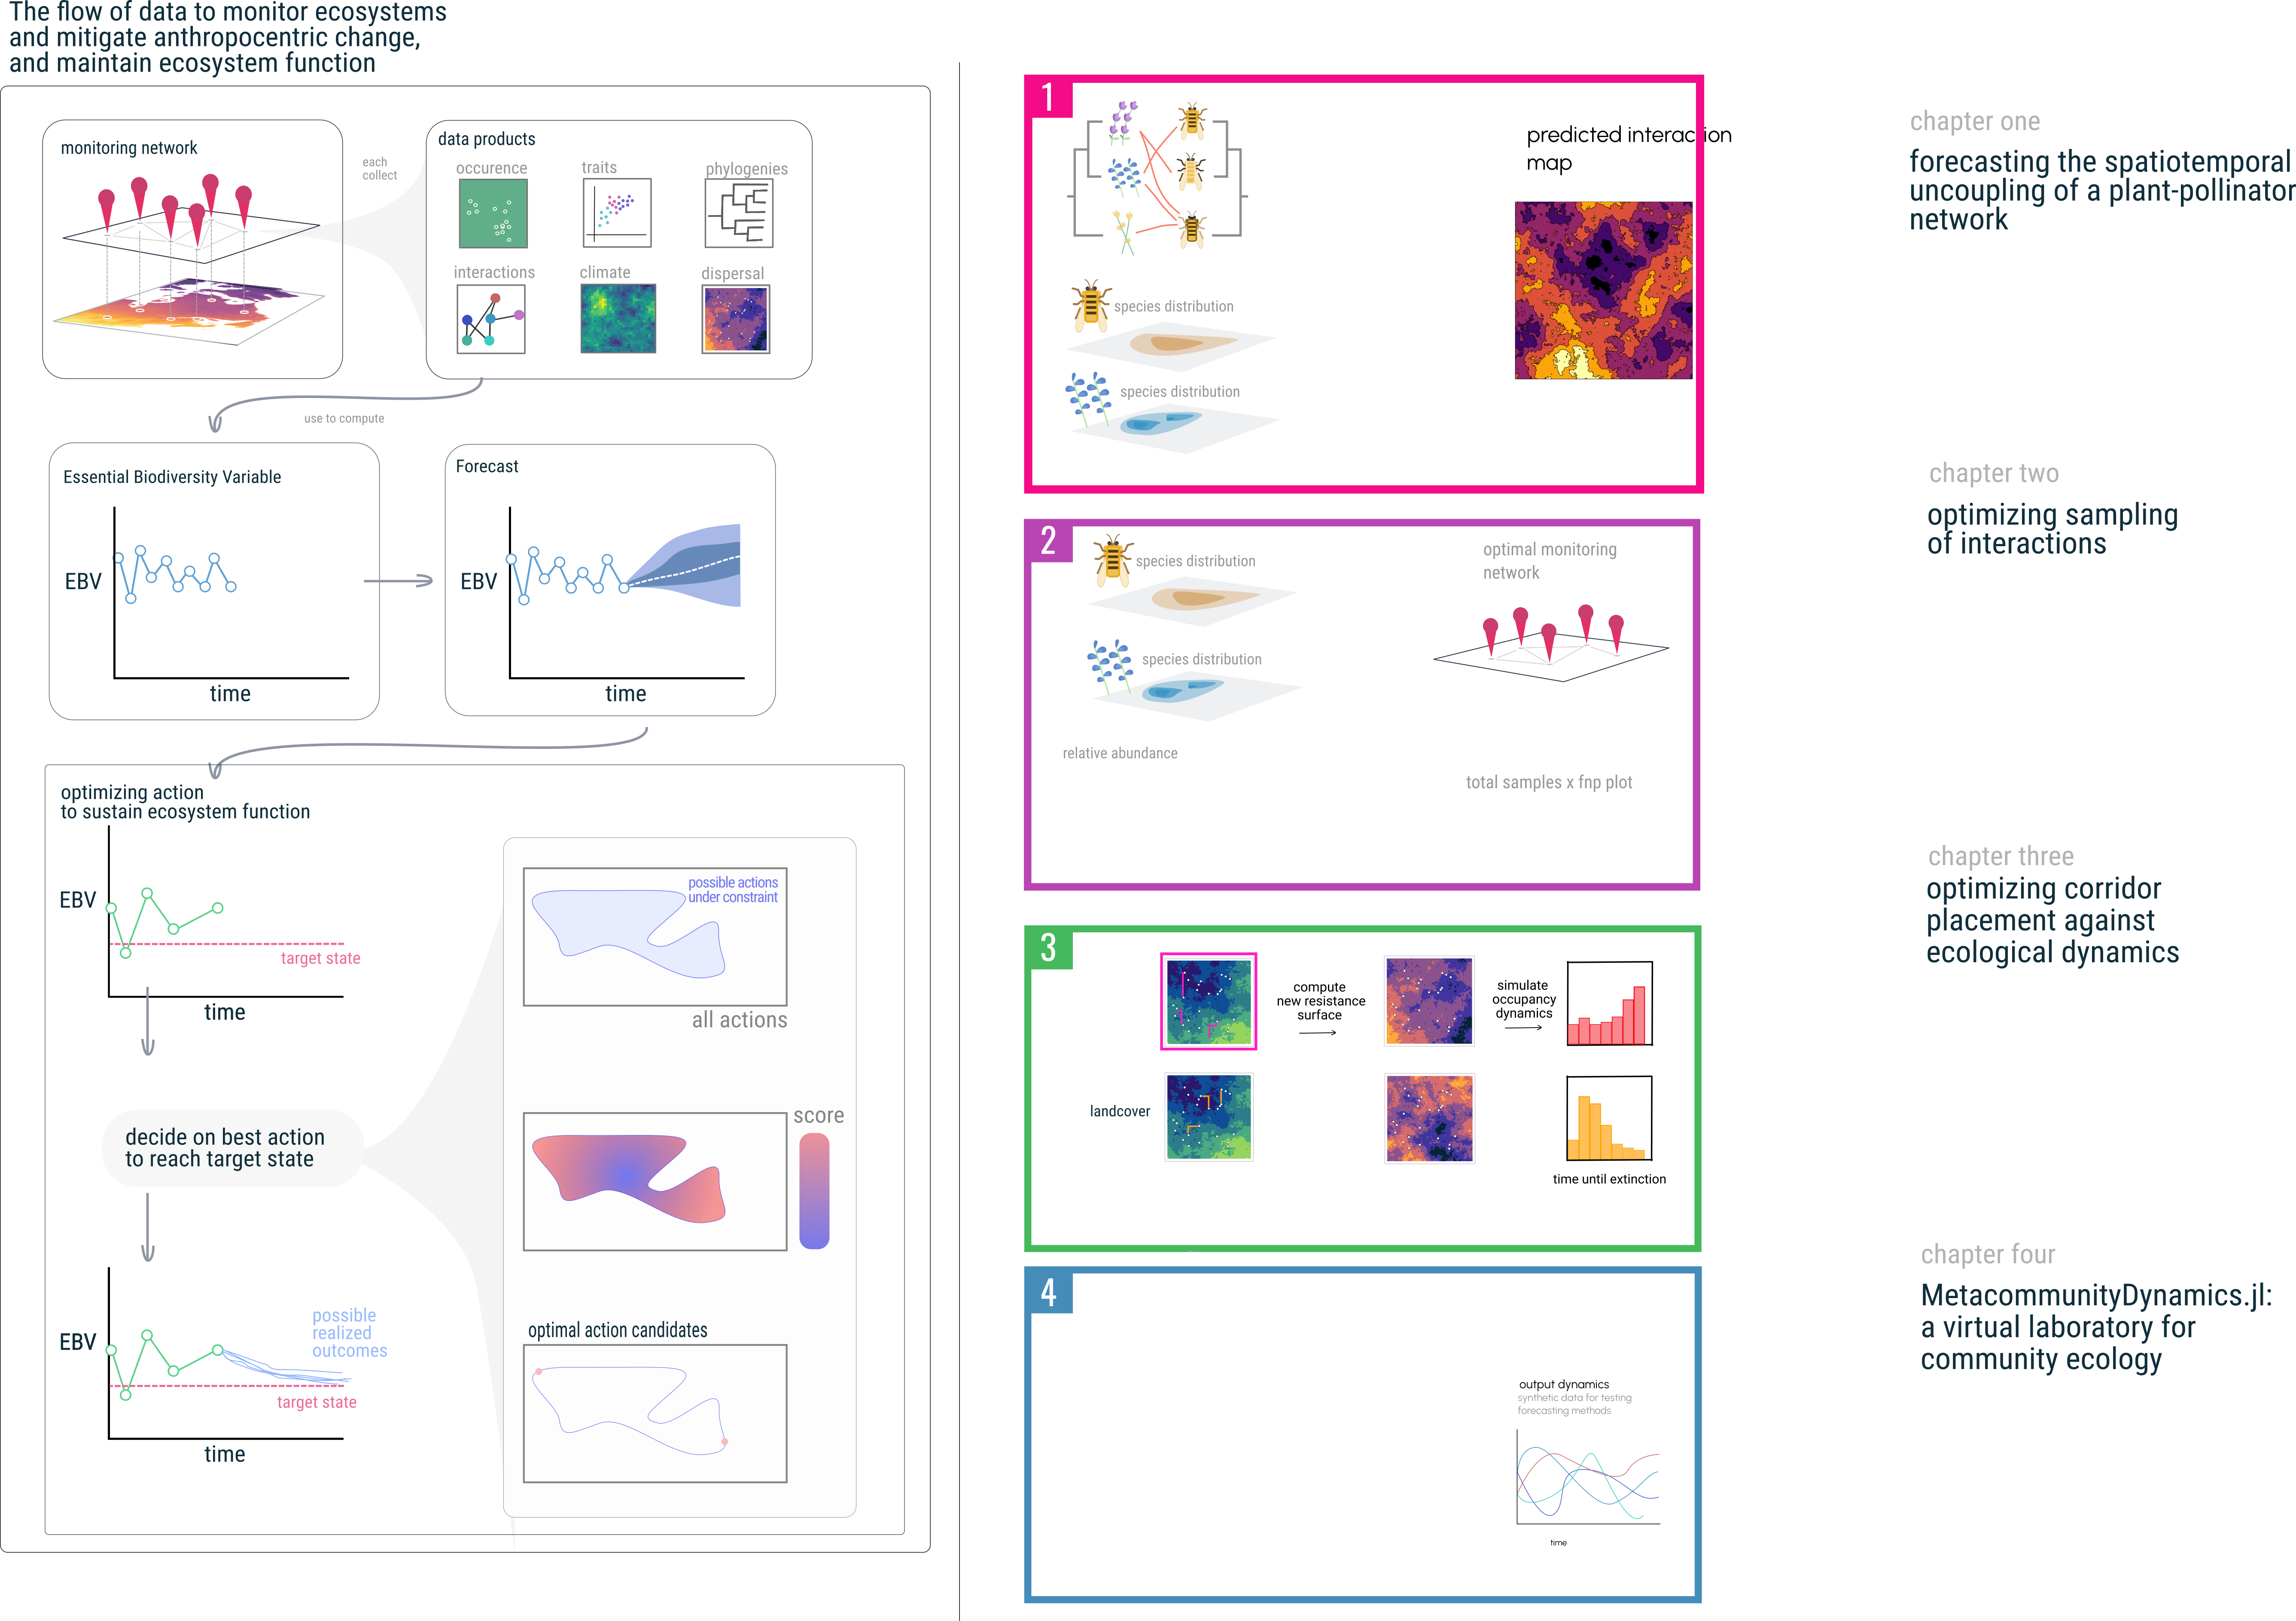
\includegraphics{./figures/thesisconcept.png}
\caption{thesis concept}\label{fig:thesis}
}
\end{figure}

The primary research challenges this thesis addresses: how do we design
ecological samples to? How do we build the software infrastructure to
assimilate data from a variety of sources? How do we propagate
uncertainty from data to forecasts? The flow of chapters follows the
flow in fig.~\ref{fig:thesis} (left), from data collection via a
monitoring network, to forecasting an essential biodiversity variable
(EBV), to optimizing mitigation strategy based on constraints. In
chapter one, we discuss how simulation can aid in the design of
ecological samples and monitoring network design. In chapter two we use
data to forecast the uncoupling of a plant-pollinator network. In
chapter three, we apply simulation methods in landscape ecology to
optimize corridor placement with respect maximize the
time-until-extinction of a metapopulation. The fourth and final chapter
is the software (\emph{MetacommunityDynamics.jl}) which enables the rest
of the dissertation.

\hypertarget{chapter-one-optimizing-spatial-sampling-of-species-interactions}{%
\section{Chapter One: Optimizing spatial sampling of species
interactions}\label{chapter-one-optimizing-spatial-sampling-of-species-interactions}}

\hypertarget{objective}{%
\subsection{Objective}\label{objective}}

This chapter uses simulation models to investigate the relationship
between species relative abundance, sampling effort, and probability of
observing an interaction between species in order to aid in the design
of samples of ecological interactions, and to provide a null expectation
of false-negative probability for a dataset of a given size. Further it
then proposes a method for optimizing the spatial sampling locations to
maximize the probability of detecting an interaction between two species
given a fixed number of total of observations, and the distributions of
each species. This addresses the optimization of monitoring network part
of the flow from data to mitigation at the top of fig.~\ref{fig:thesis},
left. As explored in the previous chapter, there are false-negatives in
interaction data. However, there is more than one way to observe a
false-negative when sampling interactions. fig.~\ref{fig:fnrtaxonomy}
shows a taxonomy of false-negatives in occurrence, co-occurrence, and
interaction data.

\begin{figure}
\hypertarget{fig:fnrtaxonomy}{%
\centering
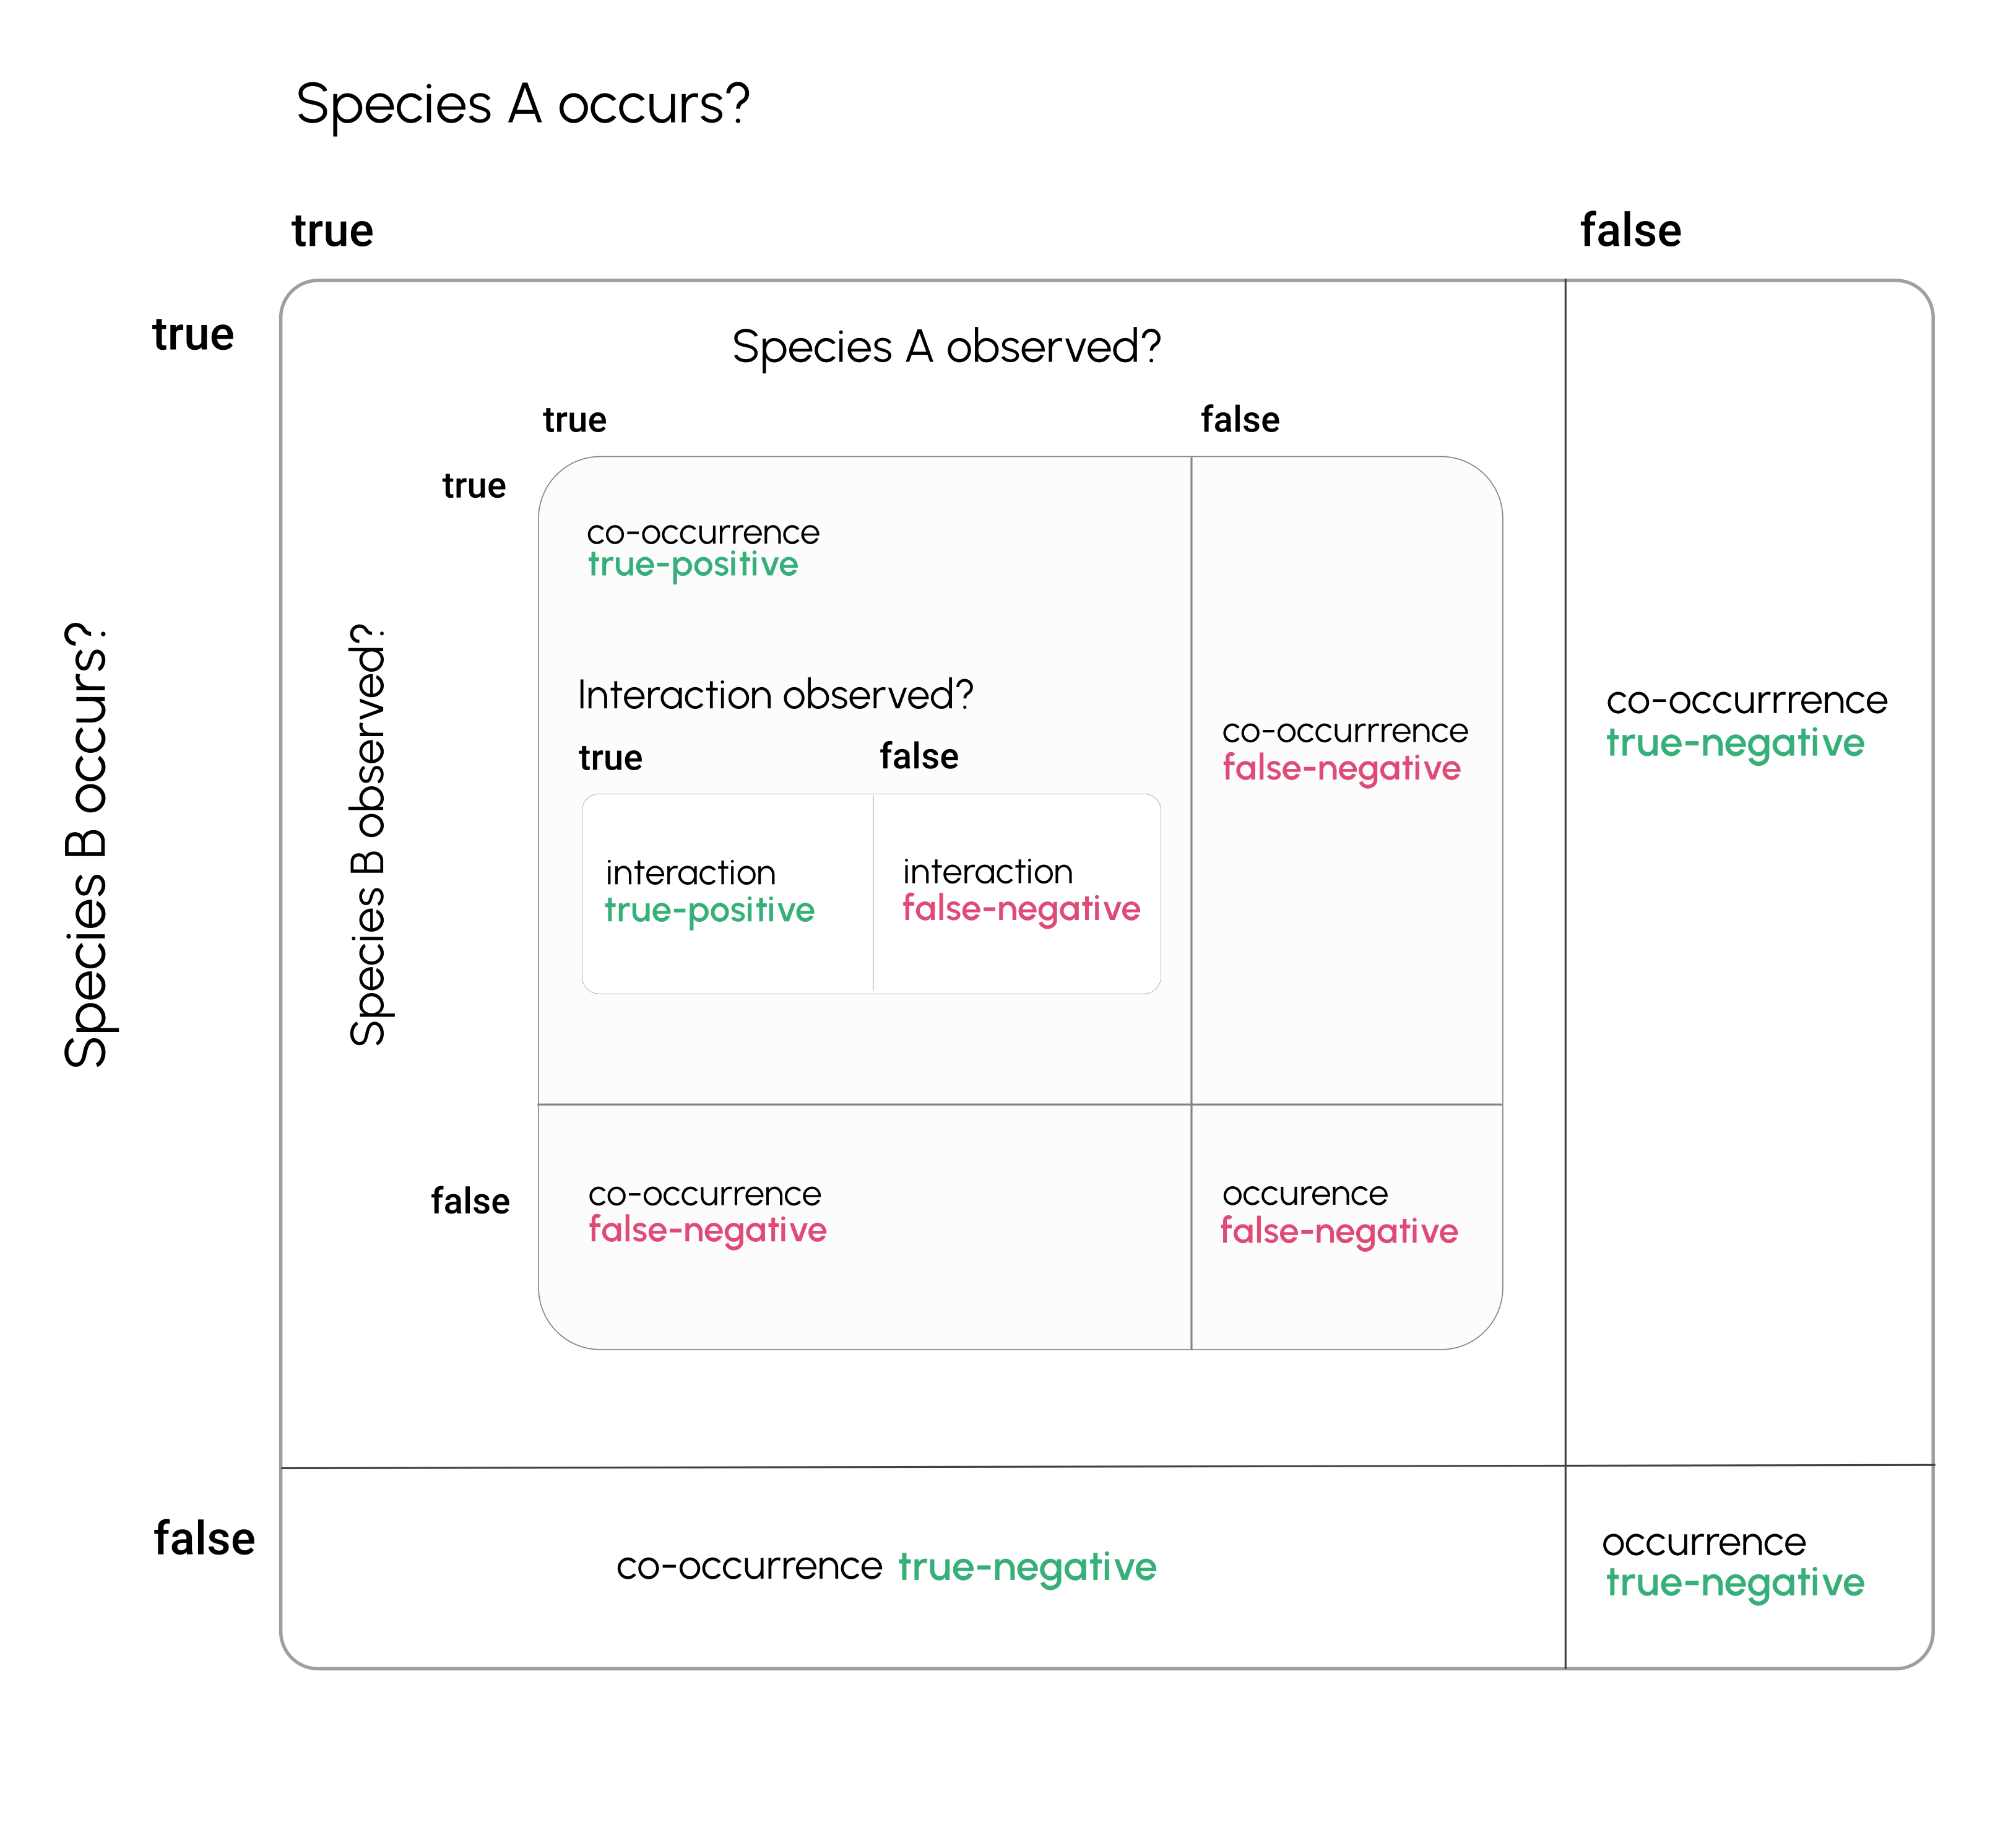
\includegraphics{./figures/ch2.png}
\caption{A taxonomy of occurrence, co-occurrence, and interaction false
negatives in data}\label{fig:fnrtaxonomy}
}
\end{figure}

\hypertarget{methods}{%
\subsection{Methods}\label{methods}}

The first result is to compute a null expectation of the probability of
an interaction false-negative as a function number of total observations
of individuals of \emph{any species}. This is done by simulating the
process of observation, where the probability of observing a given
species is its relative abundance. We use a log-normal distribution of
relative abundance (Hubbell 2001) and simulating the process of
observation on food-webs generated using the niche model (Williams \&
Martinez 2000) with connectance parameterized by the flexible-links
model (MacDonald \emph{et al.} 2020). An example of this relation for
networks with varying spceies richness is shown in fig.~\ref{fig:fnr}.

We then go on to testing some assumptions of this neutral model with
empirical data. Primarily that we analytically show that our neutral
model, if anything, underestimates the probability of false-negatives if
there are positive associations between species co-occurrence, and we
show these positive associations exist in two sets of spatially
replicated samples of interaction networks (Thompson \& Townsend 2000;
Hadfield \emph{et al.} 2014), fig.~\ref{fig:posassoc}---further I'm
planning to add the field data from the previous chapter into this
analysis once available. Finally this chapter proposes a simulated
annealing method to optimize the a set of \(n\) points in space to
maximize the probability of detecting an interaction between two species
\(a\) and \(b\) with \emph{known} distributions \(D_a\), \(D_b\).

\hypertarget{results}{%
\subsection{Results}\label{results}}

The first major result is using the simulation of the observation
process described above to generate expectations of interaction
false-negative rate (FNR) as a function of total number of observations,
with the goal being for this estimate to be used as correction for
detection error when fitting an interaction prediction model. This
relationship varies with the total richness of the metaweb
fig.~\ref{fig:fnr}.

\begin{figure}
\hypertarget{fig:fnr}{%
\centering
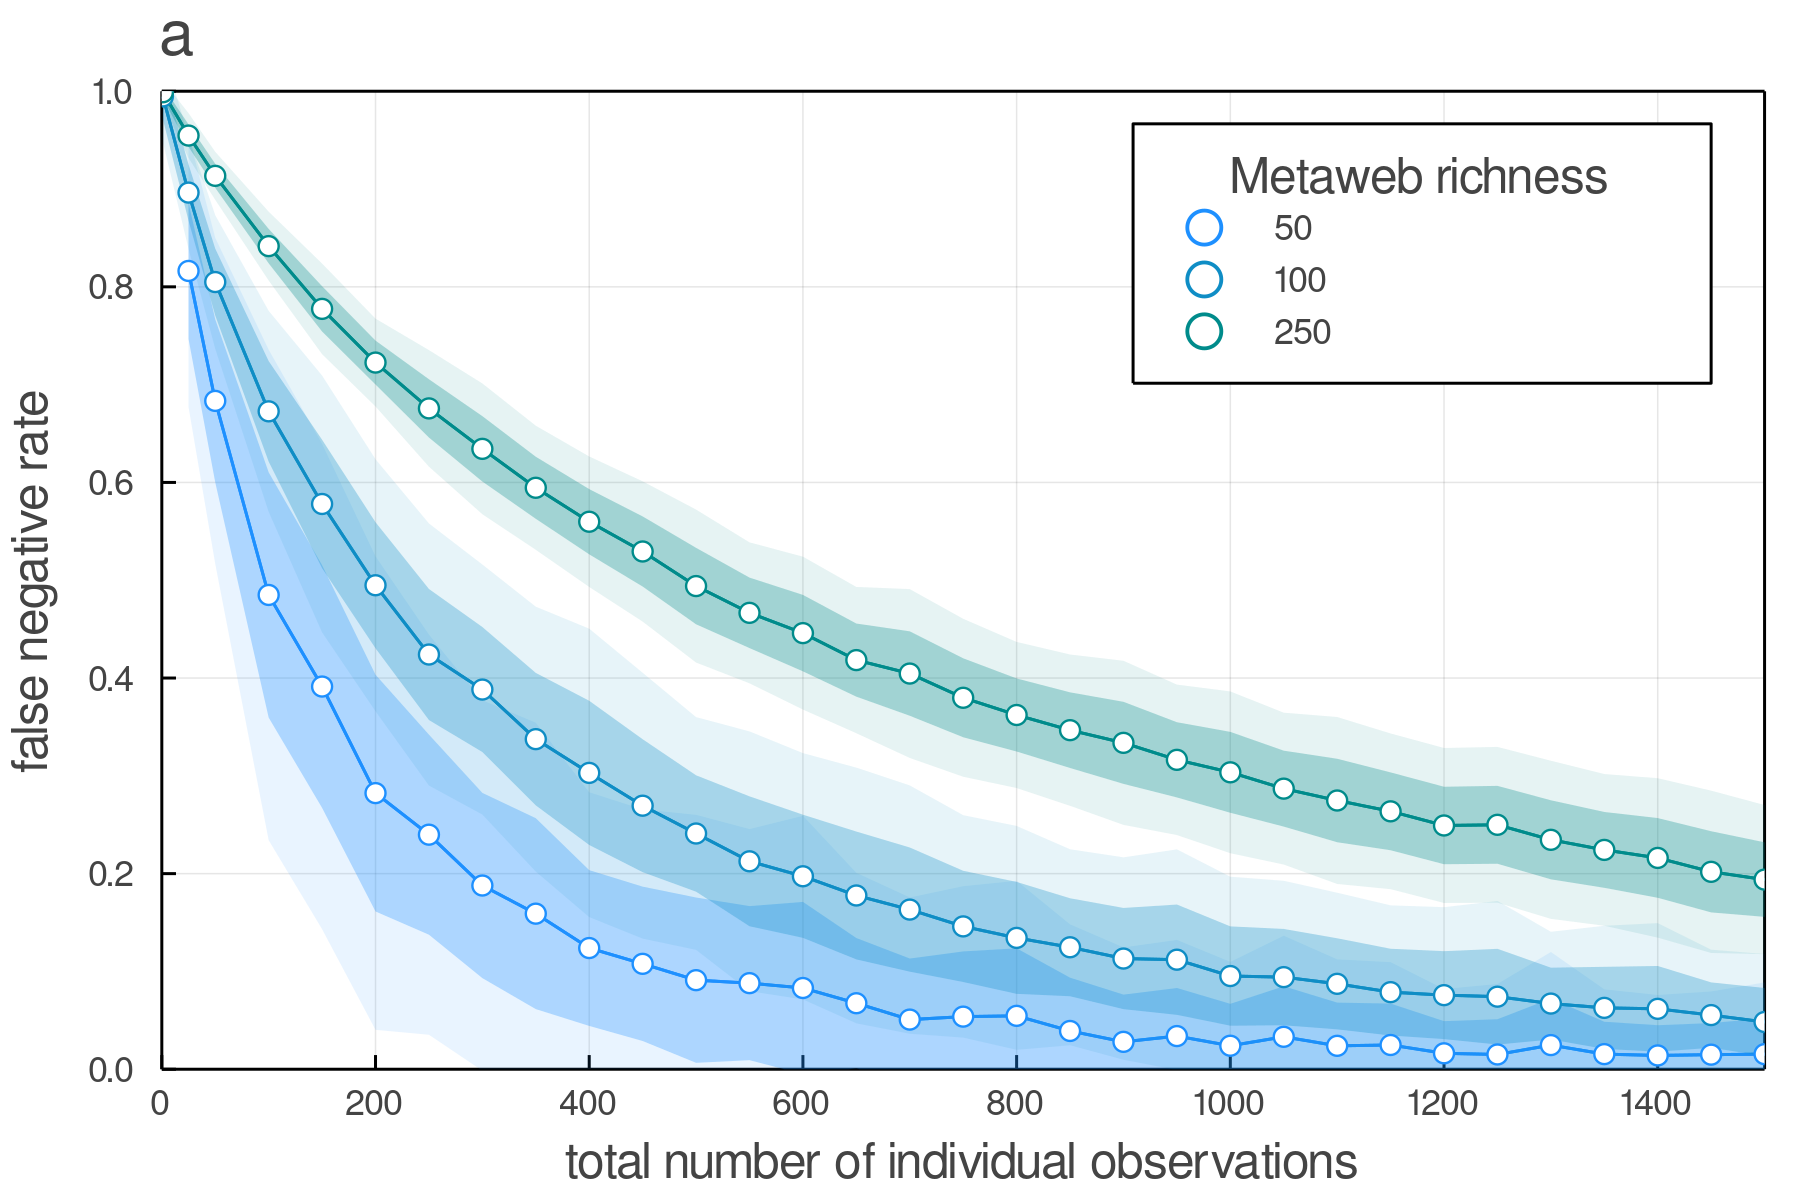
\includegraphics{./figures/ch2_fnr.png}
\caption{foo}\label{fig:fnr}
}
\end{figure}

The second major result is that we analytically show that the this
simulated observation model, by assuming that there is no association
between observing two species given that they interact, actually under
predicts the realized false-negative interaction rate. We then
demonstrate that this positive association association exists in two
empirical systems fig.~\ref{fig:posassoc}.

\begin{figure}
\hypertarget{fig:posassoc}{%
\centering
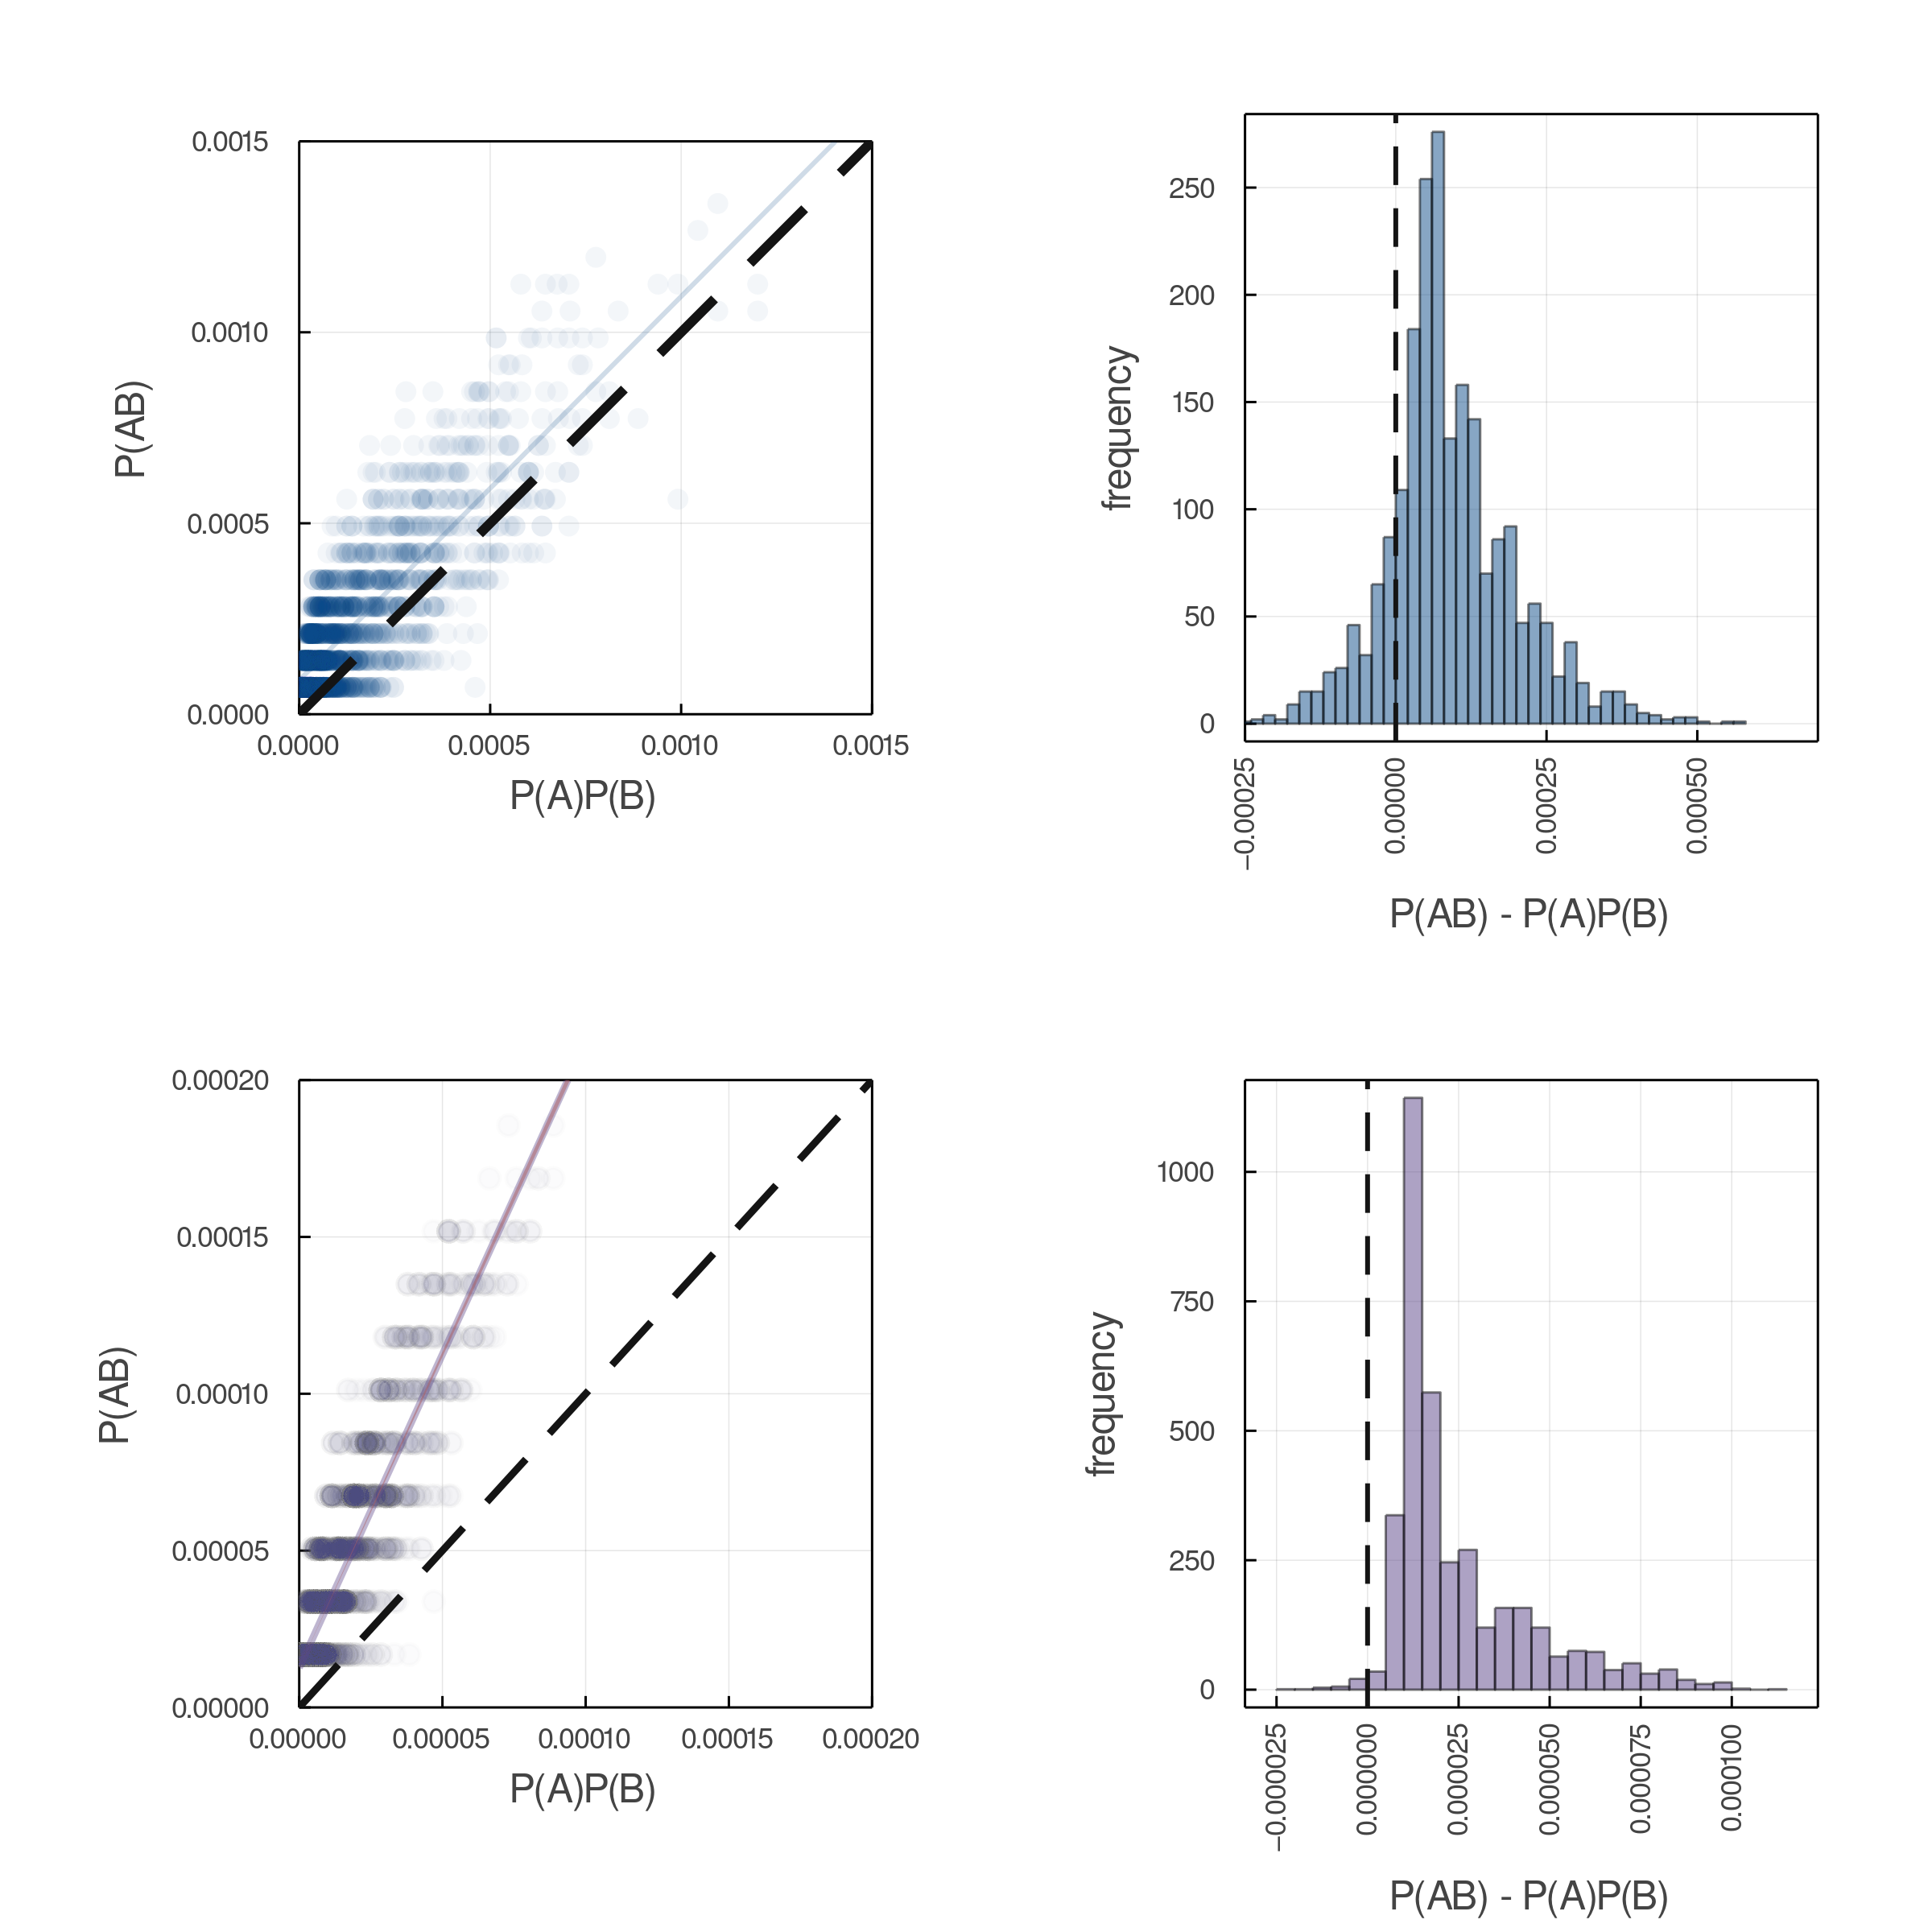
\includegraphics{./figures/positiveassociations.png}
\caption{Demonstrates positive associations in
co-occurrence}\label{fig:posassoc}
}
\end{figure}

\hypertarget{progress}{%
\subsection{Progress}\label{progress}}

This chapter is mostly complete. The only remaining work is the
implementation of simulated annealing optimization process. This will be
done by using a proposal function which takes a set of coordinates in
space and proposes a new location for each point based on a
distance-decaying kernel.

\hypertarget{chapter-two-forecasting-the-spatial-uncoupling-of-a-plant-pollinator-network}{%
\section{Chapter Two: Forecasting the spatial uncoupling of a
plant-pollinator
network}\label{chapter-two-forecasting-the-spatial-uncoupling-of-a-plant-pollinator-network}}

\hypertarget{objective-1}{%
\subsection{Objective}\label{objective-1}}

Interactions between plants and pollinators form networks which together
structure the ``architecture of biodiversity'' (Bascompte \& Jordano
2007). The functioning and stability of ecosystems emerge from these
interactions, but anthropogenic change threatens to unravel and
``rewire'' these interaction networks (CaraDonna \emph{et al.} 2017),
jeopardizing the persistence of these systems. Plant-pollinator networks
face two possible forms of rewiring in response to anthropogenic
environmental change: spatial and temporal. Range shifts could cause
interacting species to no longer overlap in space, and shifts in
phenology could cause interacting species to no longer occur at the same
time of year. This chapter uses several years of data on
bumblebee-flower phenology and interactions across several field sites,
each consisting of several plots across an elevational gradient,
combined with spatial records of species occurrence via GBIF to forecast
the uncoupling of the plant-pollinator metaweb of Colorado.

\begin{figure}
\centering
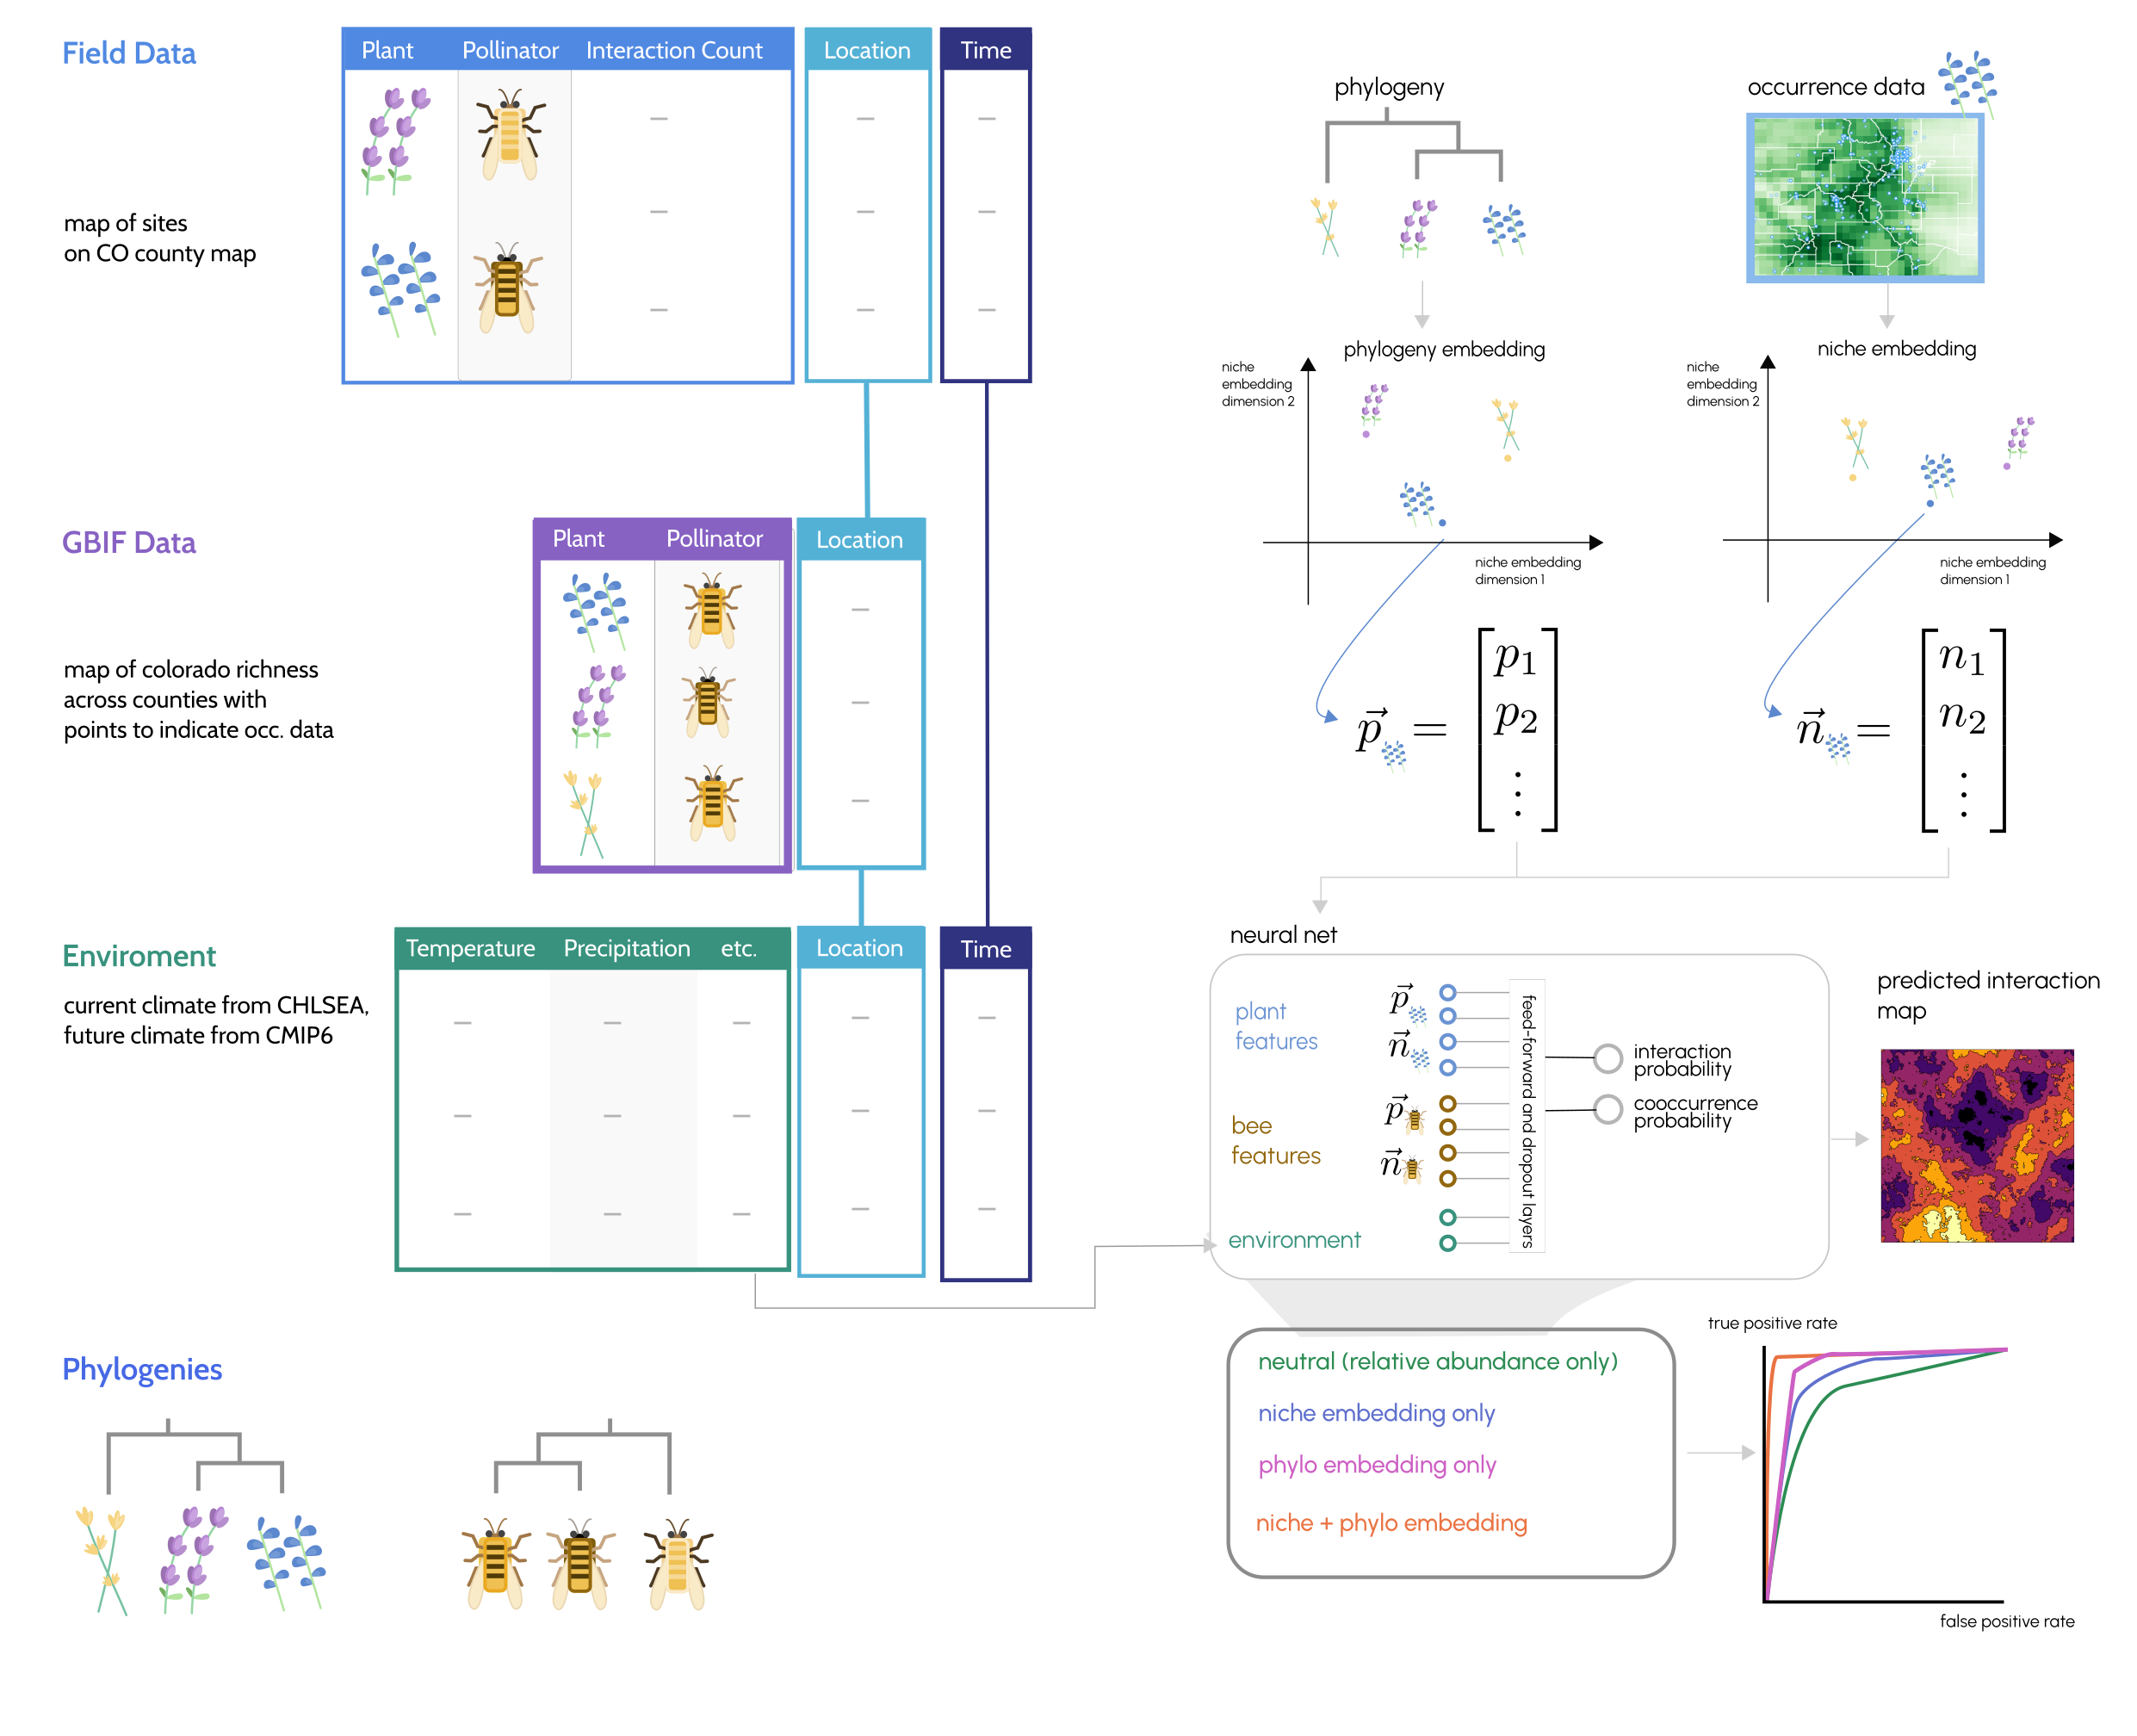
\includegraphics{./figures/ch1.png}
\caption{Chapter One conceptual figure. Left: the sources of data and
how they can be synthesized. Right: The flow from data to interaction
prediction using a few different interaction prediction models.}
\end{figure}

\hypertarget{methods-1}{%
\subsection{Methods}\label{methods-1}}

The data for this chapter is derived from multiple sources that can be
split into four categories. (1) Field data from three different field
sites across Colorado, each with multiple plots across an elevational
gradient, for seven, seven, and three years respectively. This data was
collected by Paul CaraDonna and Jane Oglevie (from the Rocky Mountain
Biological Laboratory; RMBL) and Julian Resasco (CU Boulder). (2) GBIF
spatial occurrence records of each of these species across Colorado,
including a metaweb of interactions across all of Colorado taken from
GBIF. (3) Remotely sensed data consisting of current and forecasting
bioclimatic variables from CHELSA. (4) Phylogenies for both bee and
flower species derived from NCBI GenBank barcodes for mitochondrial COI
(bumblebees) and chloroplast rbcL (flowers).

As the data we have is spatially sparse and likely to contain many
interaction ``false-negatives'' (Strydom \emph{et al.} 2021b), we begin
by predicting a metaweb of interactions across Colorado as they exist
\emph{in the present}. We do this using a set of candidate interaction
prediction models: relative abundance only, phylogenetic embedding only
(a la Strydom \emph{et al.} (2021a)), niche embedding only (Gravel
\emph{et al.} 2019), and all pairwise combinations of those constituent
models. After validating and selecting the best performing model, we
then predict how these distributions of each of these species will
change under the CMIP6 consensus climate forecast (Karger \emph{et al.}
2017), and then finally quantify the reduction in spatial between
species for which there is a predicted interaction.

\hypertarget{results-1}{%
\subsection{Results}\label{results-1}}

Here we show the in-progress results, which are the prerequisites for
the analysis outlined above: phylogenies for both plant and bee species
(fig.~\ref{fig:phylo}) and species distribution models for all species
(an example shown in fig.~\ref{fig:example_sdm}).

\hypertarget{progress-1}{%
\subsection{Progress}\label{progress-1}}

At the moment, we have derived phylogenies (fig.~\ref{fig:phylo}) and
SDMs (fig.~\ref{fig:example_sdm}) for all the species present in the
Colorado GBIF metaweb. I've also been exploring the data available from
Julian Resasco. The primary constraint on further progress is that we
are waiting on the finalization of a data sharing agreement with RMBL.

\hypertarget{chapter-three-optimizing-corridor-placement-against-ecological-dynamics}{%
\section{Chapter Three: Optimizing corridor placement against ecological
dynamics}\label{chapter-three-optimizing-corridor-placement-against-ecological-dynamics}}

\hypertarget{objective-2}{%
\subsection{Objective}\label{objective-2}}

As land-use change has caused many habitats to become fragmented and
patchy, promoting landscape connectivity has become of significant
interest to mitigate the effects of this change on Earth's biodiversity.
However, the practical realities of conservation mean that there is a
limitation on how much we can modify landscapes in order to do this. So
what is the best place to put a corridor given a constraint on how much
surface-area you can change in a landscape? This is the question this
chapter seeks to answer. Models for inferring corridor locations have
been developed, but are limited in that are not developed around
promoting some element of ecosystem function, but instead by trying to
find the path of least resistance in an existing landscape from a
derived resistance surface (Peterman 2018). This chapter proposes a
general algorithm for choosing corridor placement to optimize a
measurement of ecosystem functioning derived from simulations run on
each proposed landscape modification.

\hypertarget{methods-2}{%
\subsection{Methods}\label{methods-2}}

\begin{figure}
\hypertarget{fig:ch3}{%
\centering
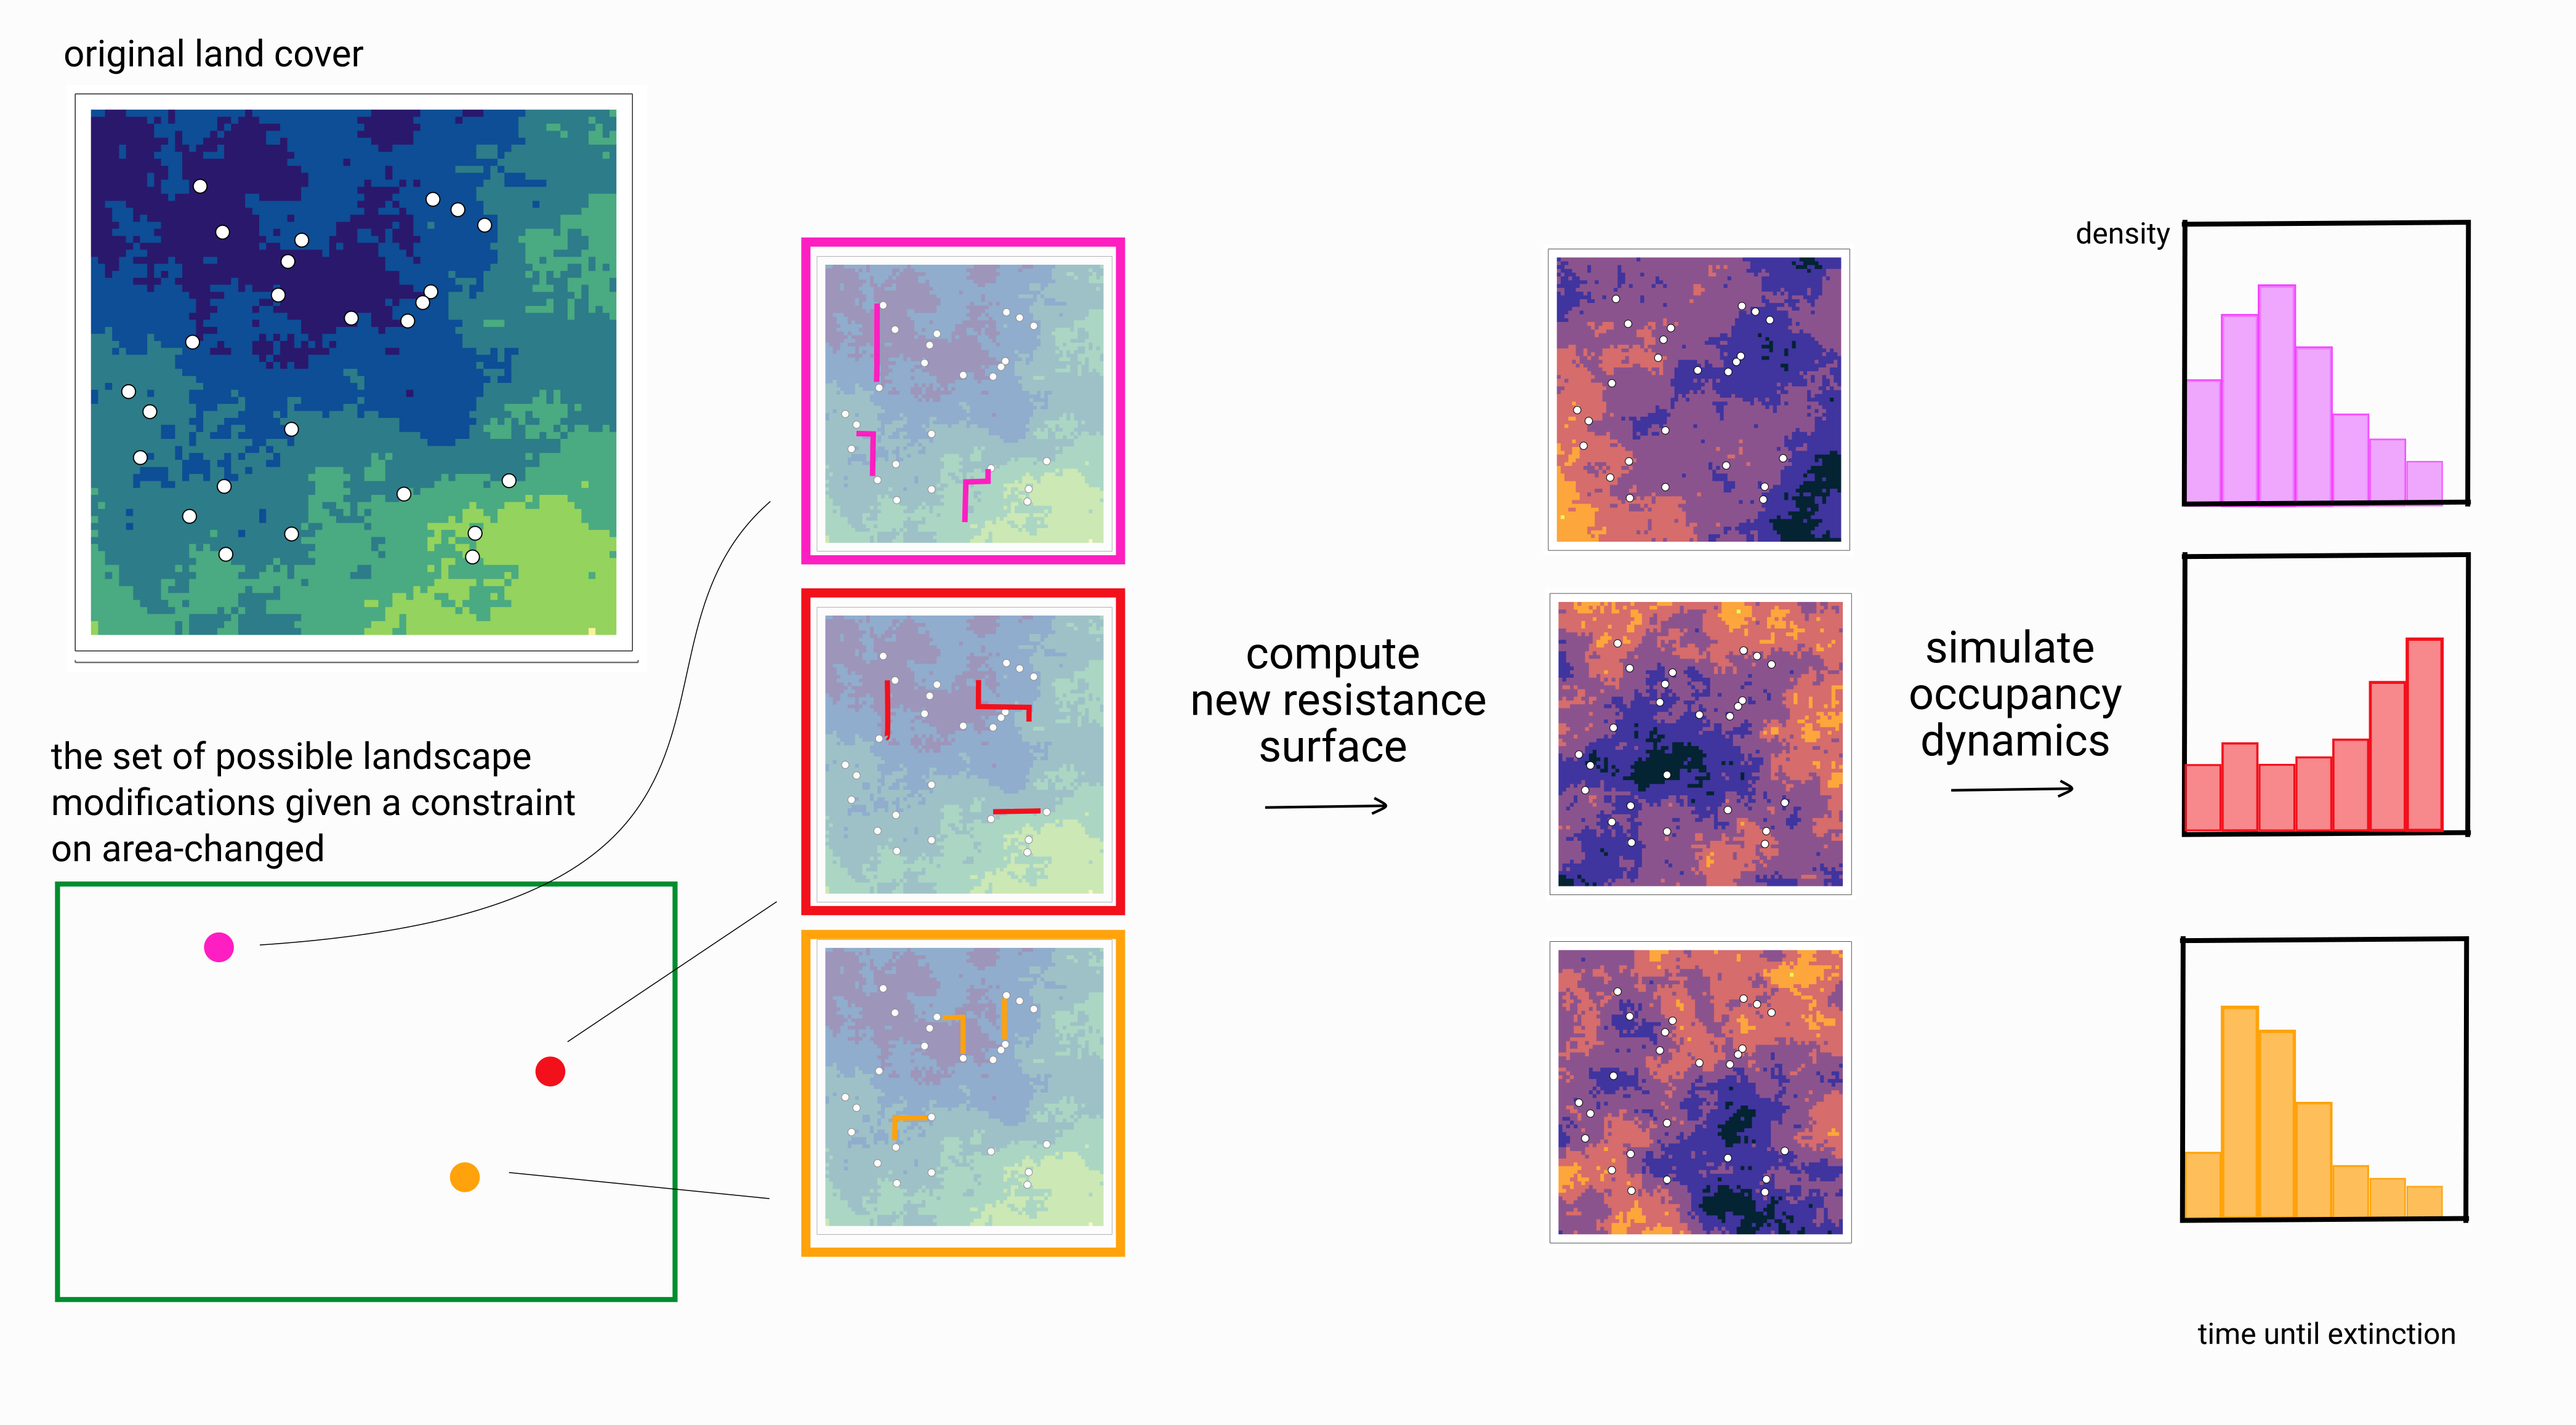
\includegraphics{./figures/ch3.png}
\caption{foo}\label{fig:ch3}
}
\end{figure}

We propose various landscape modifications which alter the cover of a
landscape, represented as a raster. We then compute a new resistance
surface based on the proposed landscape modification using Circuitscape
(McRae \emph{et al.} 2008), and based on the values of resistance to
dispersal between pair of locations we simulate spatially-explicit
metapopulation dynamics model (Hanski \& Ovaskainen 2000; Ovaskainen
\emph{et al.} 2002) to estimate a distribution of time until extinction
for each landscape modification. The largest challenge in implementing
this algorithm is the space of potential modifications grows as
\(O((nm)!)\) for an \(n\) by \(m\) raster. For most actual landscapes to
which we wish to apply this method, the set of possible modifications
becomes uncomputably large, so we use simulated annealing to explore the
search space of possible modifications to estimate the modification that
maximizes the time-until extinction of simulated metapopulation dynamics
under that hypothetical modified landscape.

\textbf{TK} The biggest challenge in implementing simulated annealing in
this context is defining a proposal function for landscape
modifications. At the moment this is done by computing the
minimum-spanning-tree (MST) of the spatial nodes, and then proposing
corridors that connect nodes that are already connected in the MST.

\textbf{TK} The goal to rank the cells in the raster by priority based
on how many times they are converted in the distribution of ``good''
corridors after simulated annealing has reached a pseudoequilibrium.
Further, the final component of this chapter is measuring the effect of
land-use change on the robustness of the optimized corridor. By
simulating various neutral models of urban and agricultural sprawl, we
can determine if the proposed modifications

\hypertarget{progress-2}{%
\subsection{Progress}\label{progress-2}}

The current progress is that I have an algorithm for proposing landscape
modifications and a simple implementation of simulated annealing. The
only gap left is implementing Circuitscape estimation of resistance
surfaces.

\hypertarget{chapter-four-metacommunitydynamics.jl-a-virtual-laboratory-for-community-ecology}{%
\section{Chapter Four: MetacommunityDynamics.jl: a virtual laboratory
for community
ecology}\label{chapter-four-metacommunitydynamics.jl-a-virtual-laboratory-for-community-ecology}}

\hypertarget{objective-3}{%
\subsection{Objective}\label{objective-3}}

The final chapter consists of a collection of modules in the Julia
language for different aspects of community ecology, including most of
the code used for the preceding chapters. Indeed
\texttt{MetacommunityDynamics.jl} (MCD.jl) is the epicenter of this set
of tools, but due to the nature of the Julia language, MCD.jl is
interoperable with serveral existing packages within the
\texttt{EcoJulia} organization, including several to which I have
contributed. We need a software library like this to generate synthetic
data from a \emph{known} set of mechanisms and parameters to test our
methods for parameter inference and forecasting on this \emph{known}
system to assess the effectiveness of these inference and forecasting
methods.

\begin{figure}
\hypertarget{fig:software}{%
\centering
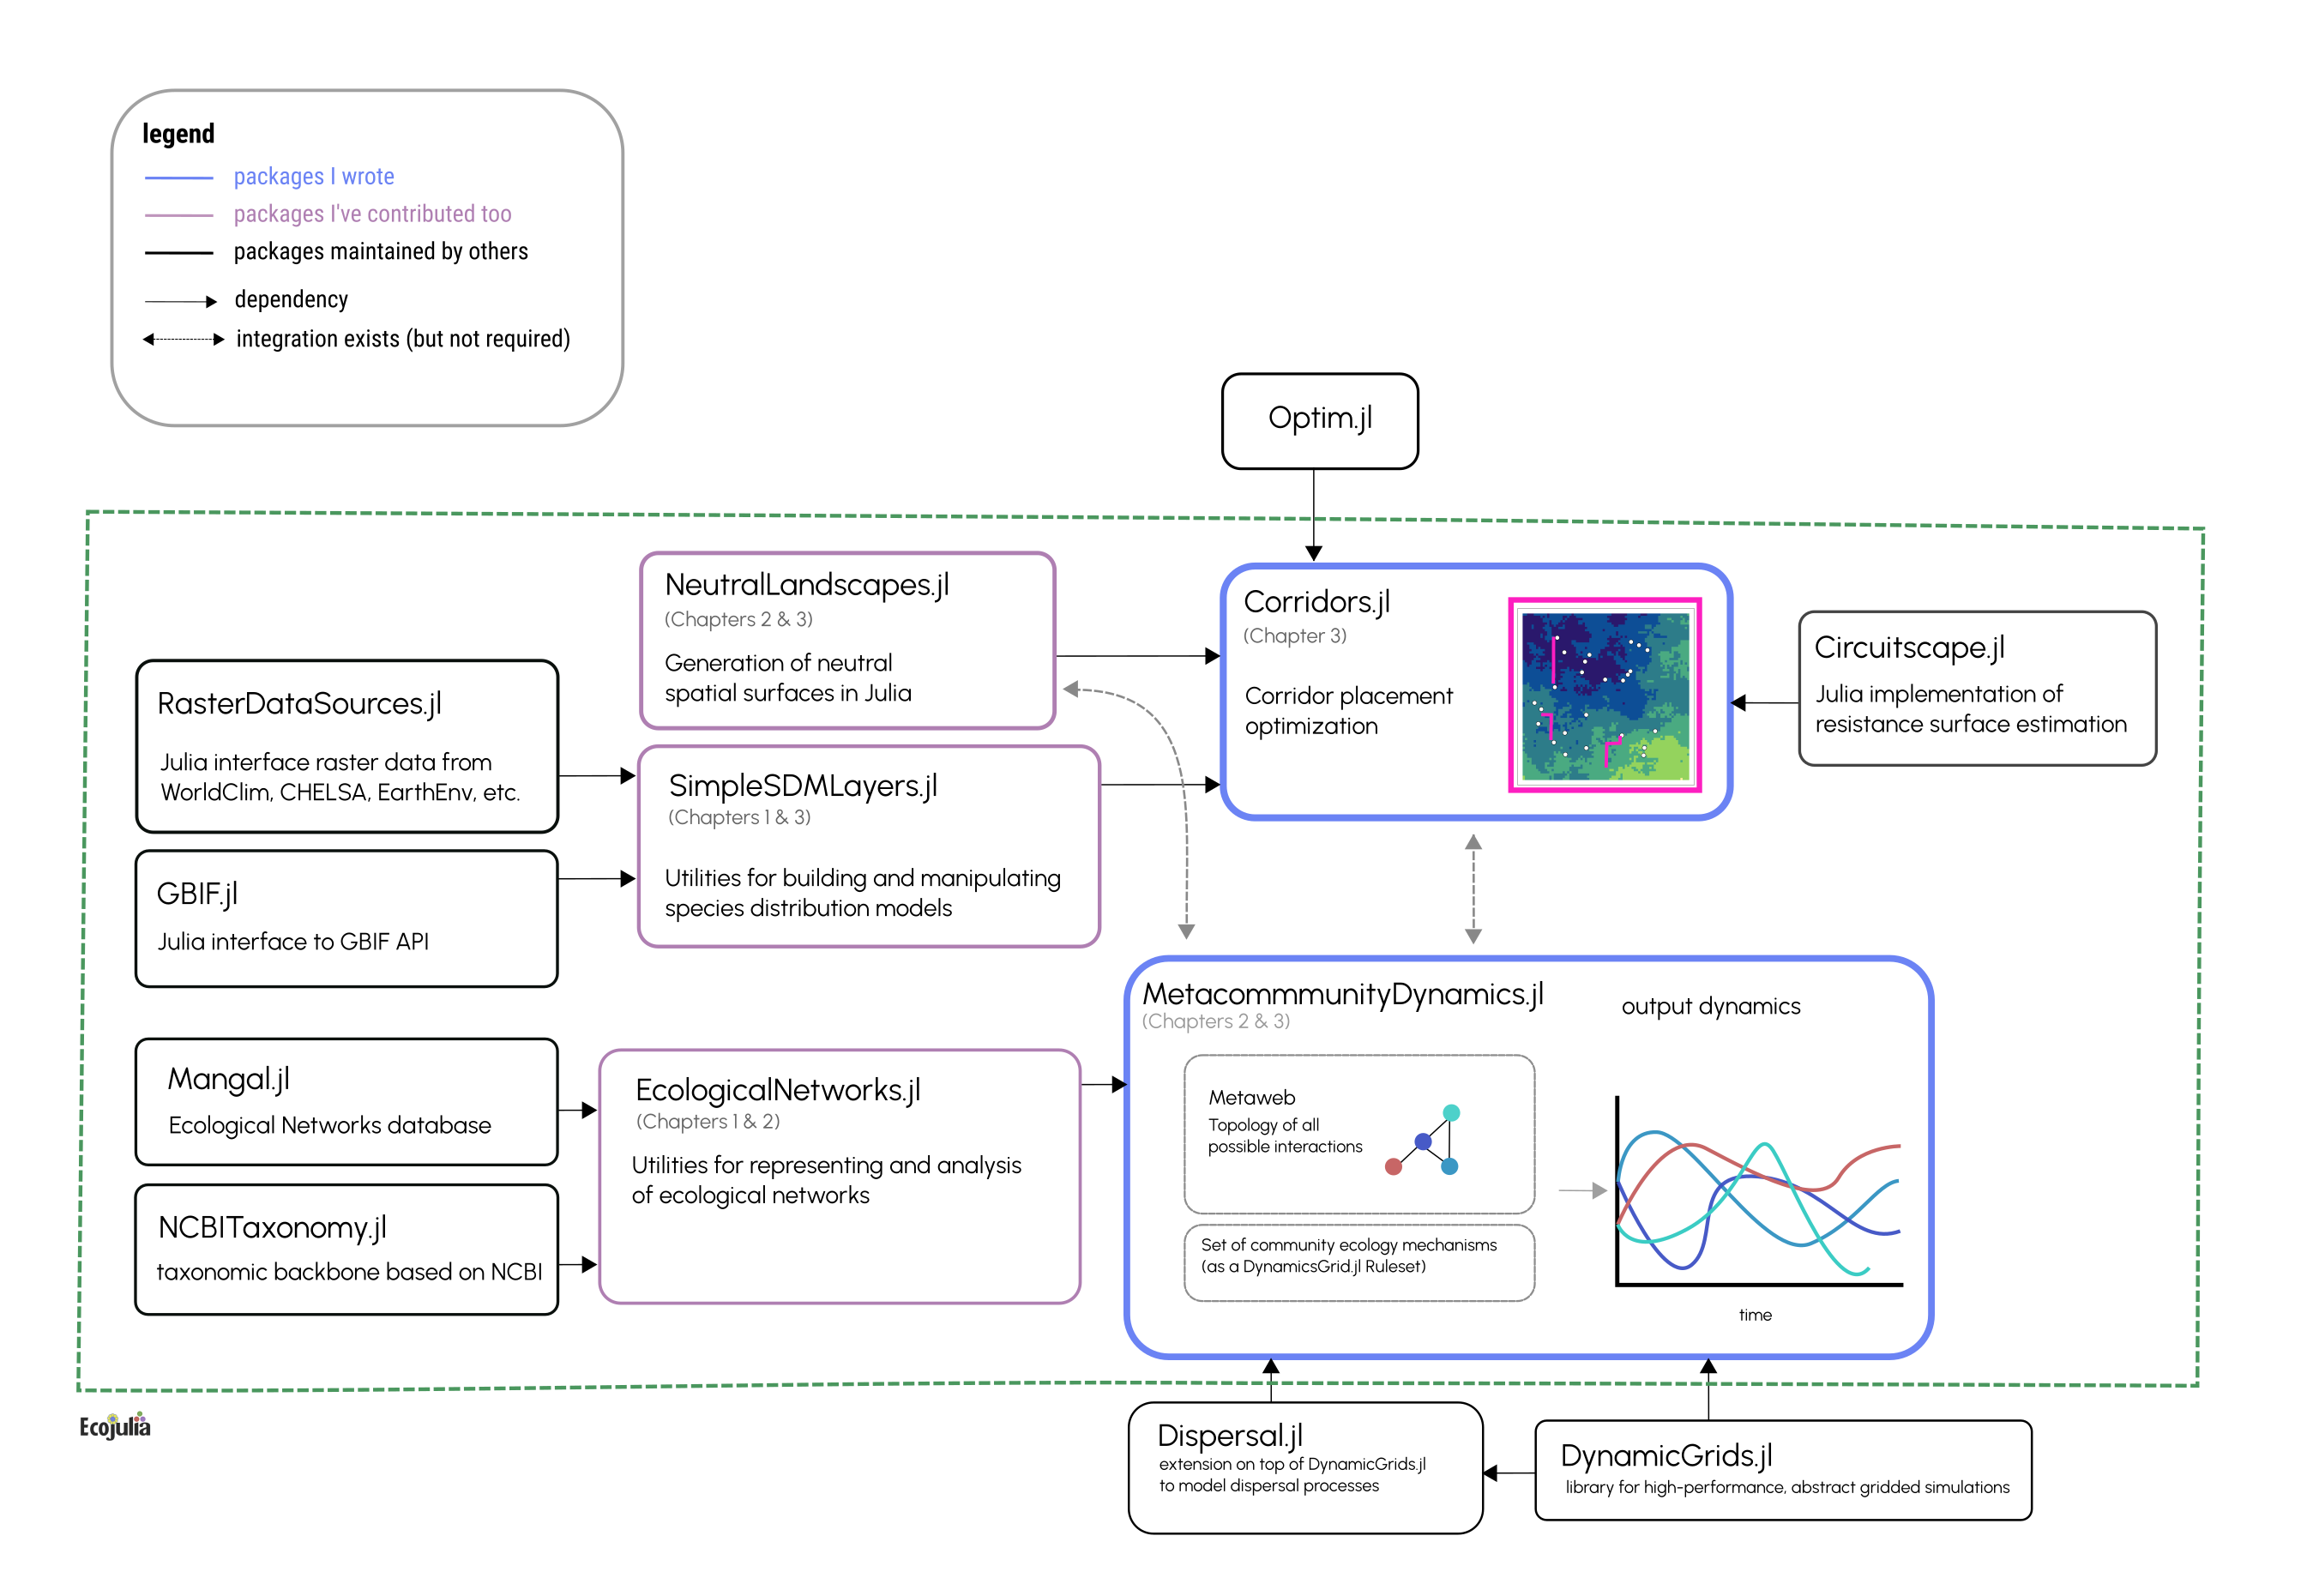
\includegraphics{./figures/ch4.png}
\caption{The structure of the software libraries used as part of
MCD.jl}\label{fig:software}
}
\end{figure}

\hypertarget{methods-3}{%
\subsection{Methods}\label{methods-3}}

A diagram showing the relation between these packages is shown in
fig.~\ref{fig:software}. \texttt{MetacommunityDynamics.jl} is built on
\texttt{DynamicGrids.jl}, a library for high-performance gridded
simulations in the \texttt{Julia} language, and Dispersal.jl (Maino
\emph{et al.} 2021), and extension of \texttt{DynamicGrids.jl}
specifically for modeling organism dispersal. It also contains
integrations with \texttt{EcologicalNetworks.jl} (Poisot \emph{et al.}
2019) to generate metawebs, or can use empirical networks from Mangal.jl
(Banville \emph{et al.} 2021). It implements the general framework for
community dynamics proposed by Vellend (2010), where all community
processes can divided into four categories: selection, dispersal, drift,
and speciation.

\hypertarget{results-2}{%
\subsection{Results}\label{results-2}}

Below (fig.~\ref{fig:foodwebtraj}) is a sample output of simulated
food-web dynamics for a metaweb of 100 species generated using the
minimum-potential-niche model with connectance \(C=0.05\) and
forbidden-link probability of \(0.5\). The dynamics change according to
a Lotka-Volttera functional response, dispersal (with dispersal distance
inverse proportional to trophic-level), linear mortality, and logistic
growth for any species at the producer trophic-level.

\begin{figure}
\hypertarget{fig:foodwebtraj}{%
\centering
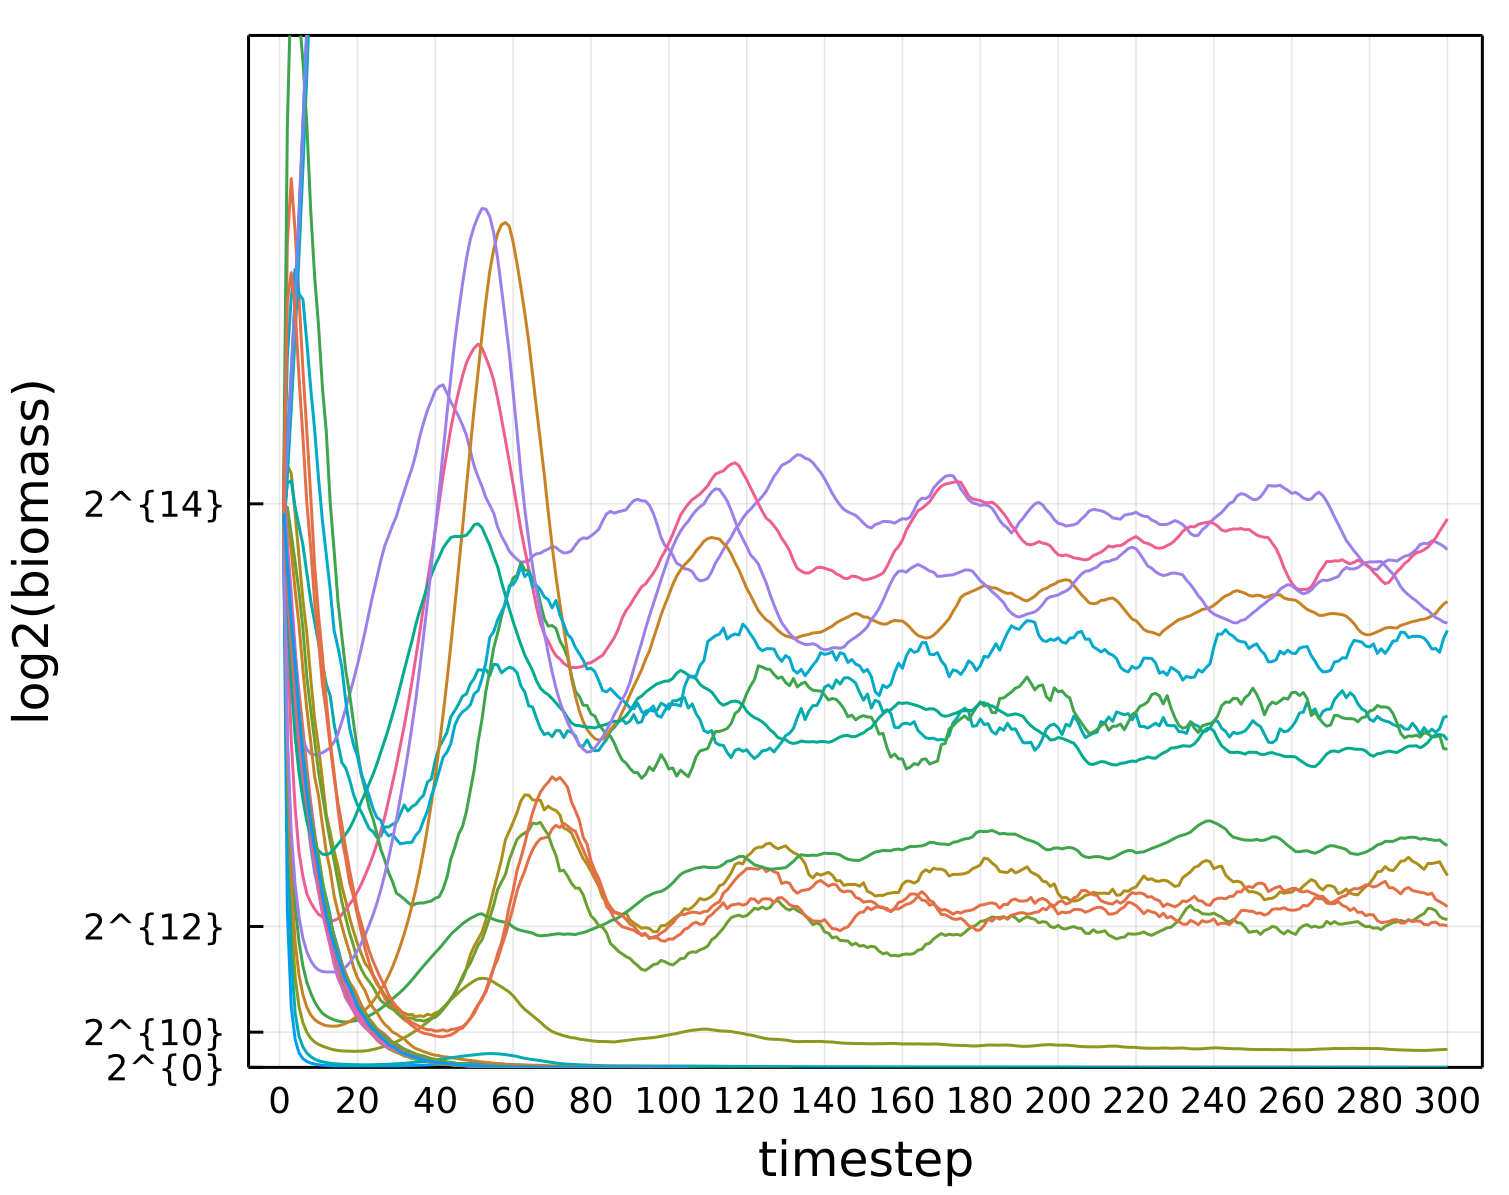
\includegraphics{./figures/foodwebtraj.png}
\caption{Sample output of simulated food web dynamics from
MetacommunityDynamics.jl}\label{fig:foodwebtraj}
}
\end{figure}

\hypertarget{progress-3}{%
\subsection{Progress}\label{progress-3}}

The software as it exists is capable of simulating the biomass dynamics
of arbitrarily large food-webs using Lotka-Volterra, Holling Type-II, or
Holling Type-III functional responses. It currently has methods to
implement Gaussian drift, and verious forms of dispersal via
Dispersal.jl. Also occupancy dynamics for Levins metapopulations (Levins
1969), and spatially explicit Hanski-Ovaskainen metapopulations (Hanski
\& Ovaskainen 2000; Ovaskainen \emph{et al.} 2002). This is most of what
needs to exist for the preceding chapters. In-progress functionality
includes selection (which affects growth-rate) on arbitrary
environmental variables in progress, as well as traits.

\hypertarget{discussion}{%
\section{Discussion}\label{discussion}}

\begin{quote}
Describing expected/anticipated contributions of the thesis. Very
important for QE. This should be at least half a page.
\end{quote}

Developing a system for global biodiversity monitoring is an imperative
to mitigate biodiversity loss and its impacts on humanity. In my thesis
I hope to provide a template for the digital infrastructure that enables
the pipeline from data collection, to forecast, to actionable
information, both through software that can be used to solve these
problems (chapters one, three, four), and vignettes of how these
software can be applied (chapters one, two).

\hypertarget{references}{%
\section*{References}\label{references}}
\addcontentsline{toc}{section}{References}

\hypertarget{refs}{}
\begin{CSLReferences}{1}{0}
\leavevmode\hypertarget{ref-Banville2021ManJl}{}%
Banville, F., Vissault, S. \& Poisot, T. (2021). Mangal.jl and
EcologicalNetworks.jl: Two complementary packages for analyzing
ecological networks in Julia. \emph{Journal of Open Source Software}, 6,
2721.

\leavevmode\hypertarget{ref-Bascompte2007PlaMut}{}%
Bascompte, J. \& Jordano, P. (2007). Plant-Animal Mutualistic Networks:
The Architecture of Biodiversity. \emph{Annual Review of Ecology,
Evolution, and Systematics}, 38, 567--593.

\leavevmode\hypertarget{ref-Bauer2015QuiRev}{}%
Bauer, P., Thorpe, A. \& Brunet, G. (2015). The quiet revolution of
numerical weather prediction. \emph{Nature}, 525, 47--56.

\leavevmode\hypertarget{ref-Beckage2011LimPre}{}%
Beckage, B., Gross, L.J. \& Kauffman, S. (2011). The limits to
prediction in ecological systems. \emph{Ecosphere}, 2, art125.

\leavevmode\hypertarget{ref-CaraDonna2017IntRew}{}%
CaraDonna, P.J., Petry, W.K., Brennan, R.M., Cunningham, J.L.,
Bronstein, J.L., Waser, N.M., \emph{et al.} (2017). Interaction rewiring
and the rapid turnover of plantpollinator networks. \emph{Ecology
Letters}, 20, 385--394.

\leavevmode\hypertarget{ref-Chen2019RevCom}{}%
Chen, Y., Angulo, M.T. \& Liu, Y.-Y. (2019). Revealing Complex
Ecological Dynamics via Symbolic Regression. \emph{BioEssays}, 41,
1900069.

\leavevmode\hypertarget{ref-Dietze2017PreEco}{}%
Dietze, M.C. (2017). Prediction in ecology: A first-principles
framework. \emph{Ecological Applications}, 27, 2048--2060.

\leavevmode\hypertarget{ref-Gravel2019BriElt}{}%
Gravel, D., Baiser, B., Dunne, J.A., Kopelke, J.-P., Martinez, N.D.,
Nyman, T., \emph{et al.} (2019). Bringing Elton and Grinnell together: A
quantitative framework to represent the biogeography of ecological
interaction networks. \emph{Ecography}, 42, 401--415.

\leavevmode\hypertarget{ref-Hadfield2014TalTwo}{}%
Hadfield, J.D., Krasnov, B.R., Poulin, R. \& Nakagawa, S. (2014). A Tale
of Two Phylogenies: Comparative Analyses of Ecological Interactions.
\emph{The American Naturalist}, 183, 174--187.

\leavevmode\hypertarget{ref-Hanski2000MetCap}{}%
Hanski, I. \& Ovaskainen, O. (2000). The metapopulation capacity of a
fragmented landscape. \emph{Nature}, 404, 755--758.

\leavevmode\hypertarget{ref-Hill2004ArcEar}{}%
Hill, C., DeLuca, C., Balaji, Suarez, M. \& Da Silva, A. (2004). The
architecture of the Earth System Modeling Framework. \emph{Computing in
Science Engineering}, 6, 18--28.

\leavevmode\hypertarget{ref-Hubbell2001UniNeu}{}%
Hubbell, S.P. (2001). \emph{The unified neutral theory of biodiversity
and biogeography}. Monographs in population biology. Princeton
University Press, Princeton.

\leavevmode\hypertarget{ref-Karger2017CliHig}{}%
Karger, D.N., Conrad, O., Böhner, J., Kawohl, T., Kreft, H., Soria-Auza,
R.W., \emph{et al.} (2017). Climatologies at high resolution for the
earth's land surface areas. \emph{Scientific Data}, 4, 170122.

\leavevmode\hypertarget{ref-Levin1992ProPat}{}%
Levin, S.A. (1992). The Problem of Pattern and Scale in Ecology: The
Robert H. MacArthur Award Lecture. \emph{Ecology}, 73, 1943--1967.

\leavevmode\hypertarget{ref-Levins1969DemGen}{}%
Levins, R. (1969). Some Demographic and Genetic Consequences of
Environmental Heterogeneity for Biological Control. \emph{Bulletin of
the Entomological Society of America}, 15, 237--240.

\leavevmode\hypertarget{ref-MacDonald2020RevLin}{}%
MacDonald, A.A.M., Banville, F. \& Poisot, T. (2020). Revisiting the
Links-Species Scaling Relationship in Food Webs. \emph{Patterns}, 1.

\leavevmode\hypertarget{ref-Maino2021PreGlo}{}%
Maino, J.L., Schouten, R. \& Umina, P. (2021). Predicting the global
invasion of Drosophila suzukii to improve Australian biosecurity
preparedness. \emph{Journal of Applied Ecology}, 58, 789--800.

\leavevmode\hypertarget{ref-Makiola2020KeyQue}{}%
Makiola, A., Compson, Z.G., Baird, D.J., Barnes, M.A., Boerlijst, S.P.,
Bouchez, A., \emph{et al.} (2020). Key Questions for Next-Generation
Biomonitoring. \emph{Frontiers in Environmental Science}, 7.

\leavevmode\hypertarget{ref-McRae2008UsiCir}{}%
McRae, B.H., Dickson, B.G., Keitt, T.H. \& Shah, V.B. (2008). Using
Circuit Theory to Model Connectivity in Ecology, Evolution, and
Conservation. \emph{Ecology}, 89, 2712--2724.

\leavevmode\hypertarget{ref-Ovaskainen2002MetMod}{}%
Ovaskainen, O., Sato, K., Bascompte, J. \& Hanski, I. (2002).
Metapopulation Models for Extinction Threshold in Spatially Correlated
Landscapes. \emph{Journal of Theoretical Biology}, 215, 95--108.

\leavevmode\hypertarget{ref-Ovaskainen2002MetMod}{}%
Ovaskainen, O., Sato, K., Bascompte, J. \& Hanski, I. (2002).
Metapopulation Models for Extinction Threshold in Spatially Correlated
Landscapes. \emph{Journal of Theoretical Biology}, 215, 95--108.

\leavevmode\hypertarget{ref-Pennekamp2019IntPre}{}%
Pennekamp, F., Iles, A.C., Garland, J., Brennan, G., Brose, U., Gaedke,
U., \emph{et al.} (2019). The intrinsic predictability of ecological
time series and its potential to guide forecasting. \emph{Ecological
Monographs}, 89, e01359.

\leavevmode\hypertarget{ref-Petchey2015EcoFor}{}%
Petchey, O.L., Pontarp, M., Massie, T.M., Kéfi, S., Ozgul, A.,
Weilenmann, M., \emph{et al.} (2015). The ecological forecast horizon,
and examples of its uses and determinants. \emph{Ecology Letters}, 18,
597--611.

\leavevmode\hypertarget{ref-Peterman2018ResRP}{}%
Peterman, W.E. (2018). ResistanceGA: An R package for the optimization
of resistance surfaces using genetic algorithms. \emph{Methods in
Ecology and Evolution}, 9, 1638--1647.

\leavevmode\hypertarget{ref-Poisot2019EcoJl}{}%
Poisot, T., Bélisle, Z., Hoebeke, L., Stock, M. \& Szefer, P. (2019).
EcologicalNetworks.jl: Analysing ecological networks of species
interactions. \emph{Ecography}, 42, 1850--1861.

\leavevmode\hypertarget{ref-Strydom2021FooWeb}{}%
Strydom, T., Bouskila, S., Banville, F., Barros, C., Caron, D., Farrell,
M.J., \emph{et al.} (2021a). Food web reconstruction through
phylogenetic transfer of low-rank network representation.

\leavevmode\hypertarget{ref-Strydom2021RoaPre}{}%
Strydom, T., Catchen, M.D., Banville, F., Caron, D., Dansereau, G.,
Desjardins-Proulx, P., \emph{et al.} (2021b). \emph{A Roadmap Toward
Predicting Species Interaction Networks (Across Space and Time)}
(Preprint). EcoEvoRxiv.

\leavevmode\hypertarget{ref-Thompson2000ResSol}{}%
Thompson, R.M. \& Townsend, C.R. (2000). Is resolution the solution?:
The effect of taxonomic resolution on the calculated properties of three
stream food webs. \emph{Freshwater Biology}, 44, 413--422.

\leavevmode\hypertarget{ref-Urban2021CodLif}{}%
Urban, M.C., Travis, J.M.J., Zurell, D., Thompson, P.L., Synes, N.W.,
Scarpa, A., \emph{et al.} (2021). Coding for Life: Designing a Platform
for Projecting and Protecting Global Biodiversity. \emph{BioScience}.

\leavevmode\hypertarget{ref-Vellend2010ConSyn}{}%
Vellend, M. (2010). Conceptual Synthesis in Community Ecology. \emph{The
Quarterly Review of Biology}, 85, 183--206.

\leavevmode\hypertarget{ref-Williams2000SimRul}{}%
Williams, R.J. \& Martinez, N.D. (2000). Simple rules yield complex food
webs. \emph{Nature}, 404, 180--183.

\end{CSLReferences}

\end{document}
